\section{Wprowadzenie}
Logiczna analiza dyskursu teologicznego nie jest może najpopularniejszą
spośród metod badawczych teorii teologicznych a prace jej poświęcone
stanowią niewielki odsetek zarówno w literaturze z dziedziny logiki i
filozofii języka, jak i teologii. Jednakże charakter badań
przedstawionych w niniejszej pracy nie jest przedsięwzięciem
odosobnionym w historii myśli. Logiką teologii w sposób systematyczny
zajmowali się już w latach trzydziestych ubiegłego stulecia
przedstawiciele tzw. Koła Krakowskiego -- Józef Bocheński, Jan
Łukasiewicz, Jan Salamucha, Jan Drewnowski oraz Bolesław
Sobociński\footnote{Zob. Z. Wolak, Naukowa filozofia koła
krakowskiego, „Zagadnienia Filozoficzne w Nauce”, nr.~36 (2005),
ss.~97-122. }. Pierwszy z nich zaznaczył się szczególnie w historii
tego typu rozważań swoją przełomową pracą \textit{The Logic of
Religion}\footnote{J.M. Bocheński, The Logic of Religion, New York
University Press, New York 1965. Pierwsze polskie wydanie: J.M.
Bocheński, Logika religii, tłum. S. Magala, Instytut wydawniczy PAX,
Warszawa 1990. W tej pracy posługuję się tym samym tłumaczeniem,
zamieszczonym w J.M. Bocheński, Logika i filozofia, Wydawnictwo Naukowe
PWN, Warszawa 1993. }. Nurt zapoczątkowany przez nich powrócił w
ostatnich latach do Krakowa jako program badawczy „logika w teologii”
prowadzony w ramach Centrum Kopernika Badań Interdyscyplinarnych.
Zaowocował on szeregiem spotkań, seminariów i konferencji, których
owocem jest wydana w 2013 roku praca zbiorowa \textit{Logic in
Theology}\footnote{B. Brożek, A. Olszewski, M. Hohol (red.), Logic in
Theology, Copernicus Center Press, Kraków 2013. }. W tej pracy będę
podążał śladami wymienionych wyżej autorów. Skupię się jednak na
szczególnej formie teologii zwanej teologią apofatyczną lub negatywną.
Jest to bardzo osobliwy rodzaj myślenia teologicznego.


Definicje:
\begin{defin}
Teologia apofatyczna -- znana także jako teologia negatywna, \textit{via
negativa} albo \textit{via negationis}, jest to teologia próbująca
opisać Boga, Boskie Dobro poprzez negację. Innymi słowy, o Bogu można
wyrażać się tylko w formach negatywnych - tzn. mówić jaki On nie jest,
a nigdy jaki jest.
\end{defin}

\begin{defin}
Teologia apofatyczna (gr. apofatikos -
,,przeczący'', nazywana też Teologią
negatywną) - nurt teologii oparty na założeniu, że jakiekolwiek
pozytywne poznanie natury Boga przekracza granice możliwości ludzkiego
rozumu. […] Teologia apofatyczna, podkreślając niewspółmierność
wszystkich poznawczych wysiłków zmierzających do opisania tajemnicy
Boga, odrzuca wszelkie symbole, obrazy i abstrakcyjne pojęcia jako
nieadekwatne do opisu natury Boga i próbuje przybliżyć Jego tajemnicę
za pomocą formuł przeczących, mówiąc, jaki Bóg nie jest. [wikipedia]
\end{defin}

\begin{defin}
Teologia apofatyczna to inna nazwa dla „teologii poprzez negację”, wedle
której Bóg jest poznawany poprzez negowanie pojęć, które mogłyby być mu
przypisane. Teologia apofatyczna podkreśla, że ludzkie pojęcia i język
są nieodpowiednim narzędziem do opisania Boga. [The Oxford Dictonary of
World Religions]
\end{defin}

\begin{defin}
Teologia Negatywna to nazwa nadana chrześcijańskiemu nurtowi\footnote{W
mojej opinii ograniczanie teologii apofatycznej do tradycji
chrześcijańskiej jest błędem. }, wedle którego Bóg jest absolutnie
transcendentny i na tyle przekracza nadawane mu nazwy i pojęcia, że w
rzeczywistości musimy je „zanegować”, by uwolnić Boga z tych ciasnych
kategorii. [Charles M. Stang]
\end{defin}

\begin{defin}
Teologia negatywna -- podobnie jak w teologii apofatycznej podejście do
Bożej Tajemnicy, które podkreśla, że raczej potrafimy powiedzieć, czym
Bóg nie jest, niż czym jest w rzeczywistości. Jest to sposób uprawiania
teologii, który kładzie większy nacisk na to, co się wyraża po łacinie
słowem sapientia (łac. „mądrość”) niż scientia (łac. „wiedza”). [Gerald
O'Collins SJ, Edward G. Farrugia SJ, Leksykon pojęć
teologicznych i kościelnych]
\end{defin}

\begin{defin}
Teologia apofatyczna -- (gr. „negatywny, przeczący”) Podstawowe pojęcie w
teologii Wschodu, często tłumaczone jako teologia negatywna. Kładzie
ono nacisk na niewspółmierność wszystkich naszych wysiłków
zmierzających do opisania absolutnej tajemnicy Boga. Każde nasze
twierdzenie o Bogu musi być ograniczone przez odpowiednie zaprzeczenie
i przez uznanie, że Bóg w sposób nieskończony przekracza wszelkie nasze
kategorie. [Gerald O'Collins SJ, Edward G. Farrugia
SJ, Leksykon pojęć teologicznych i kościelnych]
\end{defin}

Przymiotnik \textit{negativus}, który pojawia się w \textit{via
negativa} jest łacińską wersją greckiego przymiotnika
\textit{apofatikos}, pochodzącego od \textit{apofasis}, które
tłumaczone jest jako odwołanie (swoich słów), zaprzeczanie lub –
najczęściej -- jako negacja.

Mimo, iż teologia apofatyczna nigdy nie należała do głównego nurtu
teologicznego i filozoficznego myślenia o Bogu, w ciągu historii miała
całkiem pokaźne grono zwolenników.

\begin{itemize}
  \item W greckiej filozofii (prekursorzy): Platon, Plotyn, Proklos
  \item W tradycji chrześcijańskiej: Orygenes, Cyryl Jerozolimski, Ojcowie
Kapadoccy (Bazyli Wielki, Grzegorz z Nazjanzu, Jan Damasceńczyk, Maksym
Wyznawca, Jan Chryzostom, św. Jan od Krzyża, Marcin Luter.

Właściwi teologowie negatywni: Klemens Aleksandryjski, Grzegorz z Nyssy,
Pseoudo-Dionizy Areopagita, Mistrz Eckhart, Mikołaj z Kuzy, Tomasz z
Akwinu\footnote{Umieszczenie Tomasza z Akwinu wśród teologów
apofatycznych może wydać się kontrowersyjne, przemawiają jednak ku temu
pewne fragmenty jego pism. Por. P. Sikora, \textit{Logos
niepojęty.} }.

Tradycja apofatyczna jest także bardzo silna pośród wielu współczesnych
teologów prawosławnych: Vladimir Lossky, John Meyendorff, John S.
Romanides and Georges Florovsky.
  \item Pewne wątki teologii apofatycznej można odnaleźć także w tradycji
żydowskiej: Filon z Aleksandrii, Bahya ibn Paquda, Mojżesz Majmonides;
islamskiej: Ibn Arabi, Wasil ibn Ata, Avicebron; buddyjskiej i
hindusitycznej.
\end{itemize}

Teologia apofatyczna może być rozumiana jako przeciwieństwo teologii
katafatycznej (pozytywnej).


\begin{defin}
Teologia katafatyczna (gr. (\textgreek{Katafasic, katafatikoc}katafatika
- twierdzący, pozytywny, afirmacja) - , nazywana też Teologią
pozytywną. Nurt teologii oparty na założeniu, że człowiek jest w stanie
pozytywnie wypowiadać się {\textquotedbl}jaki Bóg jest{\textquotedbl}.
Teologia katafatyczna jest przeciwieństwem teologii apofatycznej.
[wikipedia]
\end{defin}


\begin{defin}
Teologia katafatyczna (gr. „twierdzący, pozytywny”) Pojęcie dopełniające
do teologii apofatycznej, czyli negatywnej, właśnie dlatego nazywane
czasami „teologią pozytywną”. Mimo że kategorie poznawcze, którymi się
kierujemy, są u samych swoich podstaw niewystarczające, możemy
wypowiadać wiele prawdziwych twierdzeń o Bogu, który się nam objawił w
sposób niezrównany w Jezusie Chrystusie i dał się nam poznać teraz
przez Ducha Świętego. Teologia apofatyczna jednak kładzie nacisk na to,
że nawet mimo faktu, iż Bóg sam siebie nam objawił i sam siebie nam
darował, pozostaje On dla nas zasadniczą tajemnicą. [Gerald
O'Collins SJ, Edward G. Farrugia SJ, Leksykon pojęć
teologicznych i kościelnych]
\end{defin}

Między tymi dwoma nurtami myślenia teologicznego istnieje wiele
odmienności. Po pierwsze, teologia negatywna dużo częściej (choć nie
zawsze) posiada charakter mistyczny, ponieważ jej negacje mają służyć
głównie do umożliwienia spotkania z transcendentnym Bogiem. Po drugie,
neguje ona nie tylko wszystkie twierdzenia dane na gruncie teologii
pozytywnej, lecz także -- krótko mówiąc -- neguje swoje własne negacje.
Tym samym teologia negatywna wydaje się być na pierwszy rzut oka
sprzeczna. By ukazać, jak wymagającym zadaniem jest zajmowane się tym
rodzajem teologii z logicznej perspektywy, posłużmy się następującym
cytatem z Pseudo-Dionizego Areopagity:




\begin{quote}
    Bóg nie jest ani duszą, ani intelektem, ani wyobrażeniem, ani
mniemaniem, ani pojmowaniem, ani słowem i pojmowaniem; […] nie jest bez
ruchu ani w ruchu, ani nie odpoczywa. […] Nie jest […] ani Boskością,
ani dobrocią […]. Nie jest też niczym z niebytu ani czymś z bytu. […]
Nie istnieje ani słowo, ani imię, ani wiedza o Nim. […] Jest ponad
wszelkim twierdzeniem i ponad wszelkim zaprzeczeniem.\footnote{
Pseudo-Dionizy Areopagita, Teologia Mistyczna, Rozdział V [w:]  Pisma
teologiczne, tłum. M. Dzielska, Wydawnictwo Znak, Kraków2005.}
\end{quote}



Jak zauważa Paweł Rojek\footnote{P. Rojek, Logika teologii negatywnej,
Pressje, nr 29 (2012), s. 216. }, wydaje się, ze Dionizy nie tylko
narusza pewne fundamentalne zasady teologii katafatycznej, lecz także
podstawowe prawa logiczne. Twierdząc, że Bóg nie jest ani niebytem, ani
bytem, Dionizy wydaje się ignorować prawa wyłączonego środka.
Oczywiście istnieją ugruntowane w literaturze i dobrze uzasadnione
filozoficznie rachunki logiczne, które odrzucają zasadę wyłączonego
środka\footnote{Do najważniejszych z nich należy logika
intuicjonistyczna. }, jednak lista naruszanych przez tego
myśliciela praw na tym się nie kończy. Twierdzenie, że Bóg nie jest
Boskością każe sądzić, że Dionizy podważa prawo tożsamości. Ponadto, w
sposób oczywisty zaprzecza samemu sobie utrzymując, że nie ma żadnego
mówienia o Bogu, podczas gdy sam się tego zadania podejmuje.

Rzeczywiście, nie ma wielkiej przesady w twierdzeniu, że teologia
negatywna jest najbardziej mistyczną, nielogiczną i niejasną teorią
Boga, jaka kiedykolwiek powstała\footnote{Tamże. }. Z tego powodu
niektórzy filozofowie, filozofowie logiki, lub teologowie mogliby
utrzymywać, że ten rodzaj teologicznego myślenia nie posiada żadnej
teoretycznej wartości a zdania takiej teologii powinny być traktowane
raczej jako modlitwa, hymn uwielbienia, wyraz czci lub środek
prowadzący do zjednoczenia z Bogiem\footnote{Takie stanowisko jest
popularne wśród myślicieli prawosławnych takich, jak Władimir Łosski.
Utrzymują je także Andrew Louth i Paul Rorem. Zob. Tamże, s. 217.
}. Mogliby oni stwierdzić, że logika formalna nie będzie w ogóle
użyteczna w wyjaśnianiu i precyzowaniu takiej teologii a każda próba
odkrycia jej logicznej struktury i formalizacji z góry skazana jest na
niepowodzenie. Na przykład Jan Woleński wprost pisze, że




\begin{quote}
    Owa teologia (negatywna) utrzymuje, że nie możemy stwierdzić niczego
pozytywnego o Bogu i jego własnościach. Powinniśmy powstrzymać się od
stwierdzeń pozytywnych i ograniczyć się do takich zdań, jak: „Nie wiem,
jaki Bóg jest, ani jaki nie jest…”. Według tego rodzaju teologii, luka
poznawcza wyłaniająca się z takich stwierdzeń jest w wystarczającym
stopniu wypełniona poprzez przekonanie rozumiane jako wiara religijna.
Jeśli wierzymy, nie musimy przejmować się oczywistymi sprzecznościami w
zbiorze zdań teologicznych. [..] Niewątpliwie, logika nie spełnia
zadniej istotnej roli teologii negatywnej, która nie jest szczególnie
zainteresowana argumentami.\footnote{J. Woleński, Theology and Logic,
[w:] Logic in Theology, red. B. Brożek et. al, Copernicus Center Press,
Kraków 2013, ss. 11-12.}
\end{quote}




W tej pracy przyjmuję odmienne stanowisko. Uważam, że także teologia
negatywna może być badana za pomocą narzędzi formalnych a wynik tego
badania może być owocny i ciekawy filozoficznie. Mimo, iż zadanie
formalizacji tego typu rozważań na pierwszy rzut oka nie wygląda zbyt
obiecująco, istnieją autorzy, którzy uznają, że teologia negatywna
posiada pewną teoretyczną (a nie tylko duchową) wartość a w literaturze
można spotkać co najmniej kilka prób zachowania spójności tej teorii.
Niektóre z tych prób wykorzystują narzędzia formalne. Wedle mojej
wiedzy, pierwszym logikiem, który próbował zmierzyć się z doktryną
teologii apofatycznej był o. Józef Maria Bocheński. Ostatecznie jednak
nie podołał on sprzecznościom, w które jest ona uwikłana i konkludował,
że należy ją odrzucić\footnote{J.M. Bocheński, Logika religii. tłum. S.
Magala, [w:]: J. M. Bocheński. Logika i filozofia. Wybór pism, PWN,
Warszawa 1993, s. 325--468. }. Niektórzy autorzy -- tacy jak np.
John J. Jones -- próbowali obronić spójność teologii apofatycznej nie
używając do tego środków formalnych\footnote{Zob. J.J. Jones, Sculpting
God: The Logic of Dionysian Negative Theology. „Harvard Theological
Review” nr 89 (1996), ss. 355–371. }.W mojej opinii, najbardziej
udaną i najciekawszą próbą logicznej analizy tego typu myślenia
teologicznego jest artykuł Pawła Rojka, „Logika teologii
negatywnej”\footnote{P. Rojek, dz. cyt. }. Przedstawia on w nim
typologię różnych interpretacji teologii Pseudo-Dionizego Areopagity i
próbuję dopasować do nich modele formalne. Praca ma charakter szkicowy
i przygotowawczy. Może ona jednak stanowić dobry punkt wyjścia dla
dalszych rozważań.


\clearpage
\section{Bocheńskiego analiza teologii negatywnej}
\subsection{Teoria tego, co niewysłowione}
Bocheński swoje rozważania na temat teologii negatywnej zawarł w dziele
\textit{Logika religii}\footnote{J.M. Bocheński, dz. cyt., s.~416-418.
 }. Przede wszystkim, odróżnia on teologię negatywną od teorii
tego, co niewysłowione. Ta ostatnia głosi, że przedmiotu religii nie da
się wyrazić, a zatem cały dyskurs religijny jest pozbawiony znaczenia.
Według wielu komentatorów teoria ta jest wewnętrznie sprzeczna. Z
reguły argumentacja za taką tezą polega na wskazaniu, że twierdząc, że
nie da się niczego powiedzieć o Bogu, teoria ta sama coś o Nim mówi, a
zatem jest sprzeczna i należy ją odrzucić. Bocheński występuje
przeciwko takiemu przedstawianiu teorii tego, co niewysłowione.
Twierdzi on, że da się ją uratować od sprzeczności, lecz nawet mimo
tego, nie odpowiada ona potrzebom dyskursu religijnego\footnote{Zob.
J.M. Bocheński, dz. cyt., ss. 353-356. }.

Bocheński uważa, że jeśli przestrzega się pewnych obowiązujących w
logice konwencji, zarzut sprzeczności stawiany teorii niewysłowionego
przestanie obowiązywać. Należałoby wpierw dowieść, że danym układzie
odniesienia teoria ta prowadzi do sprzeczności, tymczasem nikt takiego
dowodu nie przedstawił. Według Bocheńskiego jest zupełnie przeciwnie –
nietrudno wykazać, że teoria tego, co niewysłowione jest spójna.
Poniżej przedstawię jego argumentację.

Załóżmy, że dwuargumentowy predykat  $Nw(x,l)$ oznacza „$x$ jest
niewyrażalne w języku $l$”.

Zapiszmy teraz formułę zawierającą ten predykat

\begin{equation}
\exists x \exists l Nw(x, l)
\end{equation}

Wydaje się, że nie tylko można ją wypowiedzieć nie popadając w
sprzeczność, lecz także jest ona prawdziwa, nietrudno znaleźć taki
obiekt $x$ i taki język $l$, które spełniałyby zapisany wyżej warunek.
(Bocheński podaje przykład krowy i języka szachów: nie da się opisać
krowy w języku szachów).

Możemy powyższy przykład uogólnić i sformułować metajęzykową definicję
Boga o następującej postaci:

\begin{equation}\label{boch}
\forall l Nw(a, l).
\end{equation}

Na pierwszy rzut oka, wydaje się, ze ta formuła jest bardziej
problematyczna -- twierdzenie, że $x$ jest niewysłowione w żadnym języku
zdaje się prowadzić do sprzeczności. Można jednak uniknąć tego
problemu, stosując zwykłe konwencje wykorzystywane do pozbywania się
antynomii semantycznych. Należy założyć, że żadne zdanie traktujące o
pewnej klasie języków, nie jest formułowane w żadnym z tych języków.
Aby było pozbawione sprzeczności musi zostać sformułowane w innym
języku, czyli odpowiednim metajęzyku. Możemy więc założyć, że klasa
języków wspominana w \ref{boch} jest klasą języków przedmiotowych. W takim
wypadku \ref{boch} jest zdaniem metajęzyka pierwszego stopnia. Po takim
zabiegu, sformułowana definicja jest znacząca i pozbawiona
sprzeczności. Nie ma bowiem niespójności w twierdzeniu, że coś nie daje
się wysłowić w jakimś języku, lub nawet w klasie języków, o ile
twierdzenie to jest w języku nienależącym do tej klasy. Według
Bocheńskiego, przy takim założeniu, standardowym z punktu widzenia
logiki ogólnej, teoria tego, co niewysłowione pozostaje znacząca i
spójna a zarzut sprzeczności zostaje oddalony.

Bocheński odrzuca jednak teorię niewysłowionego z co najmniej dwóch
powodów. Po pierwsze, na mocy \ref{boch} nie można przypisać Bogu
jakiekolwiek własności językowo przedmiotowej. Jedyną własnością, jaką
możemy mu przypisać, jest metajęzykowa własność bycia niewysłowionym w
żadnym z języków przedmiotowych. W takim wypadku wierny, nie mógłby
akceptować żadnego zdania dyskursu religijnego, które przypisałoby Bogu
jakąkolwiek własność-przedmiotowo-językową. Wydaje się to niespójne z
faktycznym dyskursem religijnym. Po drugie, niemożliwe byłoby oddawanie
czci obiektowi, o którym wiemy tylko i wyłącznie, że nie można o nim
nic powiedzieć. Jeśli wierny miałby czcić obiekt pozbawiony własności
przedmiotowo-językowych, równie dobrze tym obiektem mógłby nie być Bóg
a szatan\footnote{Por. J.M. Bocheński, dz. cyt., ss. 354-356. }.


\subsection{Logika teologii negatywnej}
Według teologii negatywnej nie jest tak, że dyskurs religijny nic nie
znaczy, jednakże jakiekolwiek ma on znaczenie, ma je na drodze czystej
negacji. Jak zauważa Bocheński, żaden ze zwolenników teologii
negatywnej nie starał się jej sformułować dostatecznie precyzyjnie a
przez swoją niejasną postać prowokuje ona do krytyki. Większość uwag
krytycznych przedstawionych przez Bocheńskiego wskazuje na paradoksalny
charakter tej teorii.

Po pierwsze, mając wyrażenie „$x$ jest niebiałe” i stosując je w postaci
negacji do przedmiotu religii otrzymamy negację niebiałości. Będzie to
oznaczać, że przedmiot religii jest biały, a zatem otrzymamy własność
całkowicie pozytywną. Po drugie, jeśli dopuścimy do tego, by o
przedmiocie religii orzekać wszystkie negacje, popadniemy w
sprzeczność. Możemy bowiem mu przypisać własność bycia niebiałym (czyli
negację własności bycia białym) oraz własność bycia nie-niebiałym
(czyli negację bycia niebiałym), a zatem także własność bycia biały, o
ile utrzymujemy silne prawo podwójnej negacji.

Według Bocheńskiego można uniknąć tych sprzeczności, gdy ograniczy się
zakres teorii do klasy własności pozytywnych. Wpierw jednak należałoby
takie własności zdefiniować, jednakże brak jest dostatecznie
precyzyjnych definicji tego rodzaju. By uchronić teologię negatywną od
wymienionych sprzeczności a zarazem nadać jej trochę precyzji,
Bocheński proponuje następującą, indukcyjną definicję własności
pozytywnych:


\begin{enumerate}
\item Własność postrzegana bezpośrednio jest własnością pozytywną.
\item Własność definiowana za pomocą formuły zawierającej wyłącznie
symbole własności pozytywnych i terminów logiki pozytywnej jest
własnością pozytywną.\footnote{Tamże, s.~416. }
\end{enumerate}
Od razu jednak dodaje, że niniejsza definicja nie jest zadawalająca z
dwóch powodów. Po pierwsze, jest ona za szeroka -- klasa własności
pozytywnych ograniczona jest dużo surowiej, niż wymagaliby tego
zwolennicy teologii apofatycznej. Po drugie, pojęcie własności
postrzeganej bezpośrednio jest bardzo nieścisłe. Posługując się
przykładem Bocheńskiego -- dlaczego nie można by postrzegać
bezpośrednio, że krowa nie jest niebieska? Dodaje on, że przedstawione
powyżej problemy nie są najpoważniejszymi z tych które nękają teologię
negatywną. Dlatego, na potrzeby dalszych rozważań zakłada on, że
pojęcie własności pozytywnej zostało poprawnie zdefiniowane.

Bocheński próbuje podać znaczenie tej teorii w sposób formalny w taki
sposób, który zadowoliłby jej zwolenników. Niech $t$ będzie terminem
dyskursu świeckiego. Możemy wówczas utrzymywać, że znaczenie $t$ nie
stosuje się do przedmiotu religijnego. Zapis $M(t, \pi, \phi)$
oznacza „$t$ jest terminem występującym w dyskursie
świeckim w znaczeniu $\phi$”.
$\alpha$ natomiast oznacza klasę własności świeckich. Treść zdań wiary
przybierze zatem następującą postać:

\begin{equation}\label{boch2}
   M(t, \pi, \phi) \land
\phi \in \alpha
\to \neg \phi (PR),
\end{equation}
gdzie $PR$ oznacza przedmiot religii, czyli Boga. Wówczas dyskurs
religijny zawiera tylko twierdzenia, które orzekają o Bogu negację
własności pozytywnych wyrażone w terminach świeckich. Dzięki
ograniczeniu teorii do klasy własności pozytywnych, tak sformułowana
teologia negatywna nie zawiera sprzeczności. W przeciwieństwie do
formalizmu użytego w teorii tego, co niewysłowione nie jest to własność
metajęzykowa, lecz własność przedmiotowo-językowa drugiego stopnia.
Jednakże, podobnie jak w teorii tego, co niewysłowione, nie możemy
przypisać Bogu żadnej własności przedmiotowo-językowej pierwszego
stopnia. Z tego powodu dzieli ona te same te same wady, co teoria
niewysławialnego. Nawet, jeśli jest niesprzeczna, nie jest zgodna z
dyskursem religijnym i praktyką religijną. Nie można czcić czegoś,
czemu nie można przypisać żadnej własności pozytywnej. Z tego powodu
powinna zostać odrzucona\footnote{Zob. tamże s.~417-418. }.

\clearpage
\section{Logika teologii negatywnej według Gellmana}

Jerome I. Gellman\footnote{Zob. J.I. Gellman, The Meta-Philosophy of Religious Language,
"Nous", nr 11 (1971), ss.~151--161.}
 ocenia adekwatność różnych analiz znaczenia języka religijnego.
Uważa on, że analizy te powinny być uporządkowane nie ze względu na to,
jak wiele z języka religijnego mogą objąć, lecz ze względu na to,
których jego elementów dotyczą. Zdania języka religijnego nie mają
równego statusu. Jedne z nich są bardziej istotne od drugich. Np. w
przypadku tradycji chrześcijańskiej, najważniejszym fragmentem języka
religijnego są teksty biblijne i pisma Ojców Kościoła. Na tej podstawie
Gellman wyróżnia on dwa rodzaje problemów teologicznych: zewnętrzne i
wewnętrzne. Przykładem pierwszego jest niezgodność twierdzenia o
wszechwiedzy Boga (w szczególności wiedzy dotyczącej przyszłości) z
tezą o wolnej woli. Zagadnienie to nie pojawia się w podstawowych
tekstach chrześcijańskich czy judaistycznych -- zostało wypracowane
dopiero przez filozofów scholastycznych, którzy te teksty komentowali.
Przykładem religijnego problemu wewnętrznego jest twierdzenie o
wszechmocy, wszechwiedza i dobroci Boga w obliczu tego, że na świecie
istnieje niesprawiedliwość. Według Gellmana każda adekwatna analiza
języka religijnego nie powinna usuwać wewnętrznych problemów danej
religii.

Gellman rozważa krótko kazus teologii negatywnej. Kojarzy ją jednak
wyłącznie z teologami żydowskimi i arabskimi\footnote{Wśród podanych
przez niego przykładów teologów negatywnych pojawia się Mojżesz
Majmonides, Abraham Ibn Daud oraz Bahya Ibn Pakuda. }. W jego
rozważaniach teologia negatywna jest teorią, w której jakikolwiek
predykat P języka „skończonych bytów” nie może być przedziwie orzekany
o Bogu. Na potrzeby tych rozważań Gellman definiuje zakres gatunkowy
predykatu P jako dziedzinę obiektów, o których można orzec P albo jego
dopełnienie. W świetle tej definicji, główną tezą teologii negatywnej
jest, że Bóg nie należy do zakresu żadnego z predykatów naszego języka.
Jeśli mówimy na przykład, że Bóg nie jest mądry, mamy na myśli raczej
negacje \textit{wykluczającej}, niż negację \textit{wyboru}. Naszym
zamiarem stwierdzenie tylko, że to nieprawda, że predykat P przysługuje
Bogu, niekoniecznie sugerując jednocześnie, że można o nim orzec
dopełnienie tego predykatu. Bóg jest poza jego gatunkowym zakresem, to
znaczy, że nie należy do zbioru obiektów, o których można orzec $P$ lub
nie-$P$. Gellman dodaje, że jeśli traktujemy istnienie jako kwantyfikator
a nie jako predykat, stwierdzenie istnienia Boga polega na stwierdzeniu
istnienia obiektu poza rodzajowym zakresem wszystkich naszych
predykatów. Zdanie to można zapisać następująco:

\begin{equation}\label{gellman}
    \exists x \forall P \neg
(P(x) \lor \neg P(x))
\end{equation}


Według Gellmana, zdanie „Bóg jest potężny” teolog negatywny zrozumie
jako negację dopełnienia predykatu „jest potężny”. W innym kontekście
oznaczałoby to przypisanie obiektowi, o którym mowa, tej właśnie
własności. Jednakże w przypadku Boga negowanie dopełnienia predykatu P
nie oznacza przypisywania mu P, ponieważ dopełnienie dane jest innym
rodzajem negacji -- negacją wykluczającą. Mówiąc ogólnie, zdania języka
religijnego negują dopełnienia wszystkich wymienianych przez nie
własności Boga, który jest poza zakresem wszystkich naszych predykatów.
One, z kolei -- będąc predykatami języka skończonych bytów -- z
konieczności muszą oznaczać niedoskonałe własności.

W końcu, Gellman odrzuca teologię negatywną, jako teorię nieadekwatną.
Po pierwsze, ze względu na wynikającą z niej niepoznawalność Boga. Po
drugie, dlatego, że w ramach tej teorii nie można postawić wewnętrznych
problemów teologicznych. Na przykład mówienie o wszechmocy,
wszechwiedzy i dobroci Boga -- w interpretacji Gellmana -- oznacza
jedynie, iż nie przypisujemy mu takich własności, jak słabość, głupota
czy moralna niedoskonałość. Nie twierdzimy przy tym, że można o nim
orzekać takie predykaty, jak moc wiedza czy dobroć. W takim wypadku nie
ma mowy o problemie wynikającym z obecnej w świecie niesprawiedliwości.

\clearpage
\section{Teologia apofatyczna w rozważaniach Jonesa}

Jones, podobnie jak Rojek, analizuje bezpośrednio teksty
Pseudo-Dionizego Areopagity. Zadaniem, jakie sobie stawia, jest
stawienie czoła sprzecznościom uwikłanym w jego doktrynę. Analizuje on
fragmenty różnych prac Dionizego po to, by właściwie zinterpretować
niejasne wyrażenia zawarte w \textit{Teologii mistycznej} i odsłonić
logiczną strukturę jego apofatycznej wykładni. Sugeruje on, że głównym
celem Dionizego było zaprzeczenie, że Bóg należy do kategorii bytów.
Próbuje też wskazać, że wbrew powszechnemu mniemaniu, teologia
negatywna nie jest teorią logicznie spójną.

Według Jonesa, teologia dionizyjska jest w dużej mierze teologią
krytyczną. Polemizuje ona z błędnym sposobem mówienia o Bogu -- takim,
który traktuje Go jak inne byty, czyli rzeczy lub pojęcia. W
\textit{Teologii mistycznej} Dionizy pisze:

\begin{quote}
    that is to say, to those caught up with the things of the world, who
imagine that there is nothing beyond instances of individual being and
who think that by their own intellectual resources they can have a
direct knowledge of him who has made the shadows his hiding place. And
if initiation into the divine is beyond such people, what is to be said
of those others, still more uninformed, who describe the transcendent
Cause of all things in terms derived from the lowest orders of being,
and who claim that it is in no way superior to the godless, multiformed
shapes they themselves have made?\footnote{Pseudo-Dionizy Areopagita,
Teologia Mistyczna, rozdział I.}
\end{quote}


Według Areopagity, bałwochwalcy mylą Boga z przedmiotami, zaś inni
„niedoinformowani”, prawdopodobnie środkowi platonicy, z pojęciami. W
innym tekście próbuje przedstawić, jak ci ostatni mogliby krytykować
wykorzystywanie materialnych obrazów do przestawienia Boga, preferując
raczej łączenie Boga z pojęciami:


\begin{quote}
    It could be arguedt hat if the [scripturew riters wantedt o
givecorporeal form to what is purely incorporeal, they. . . should have
begun with what we would hold to be noblest, immaterial and
transcendent beings [for instance, Word and Mind].\footnote{Tenże,
Hierarchia niebiańskia, rozdział II.}

Now these sacreds hapesc ertainlys how morer everencea nd seem vastly
superior to the making of images drawn from the world. Yet they are
actually no less defective than this latter, for the Deity is far
beyond every manifestationo f being and of life. . . every reason or
intelligence falls short of similarity to [the Deity].\footnote{Tamże.}
\end{quote}

Dionizy zgadza się z filozoficznym podejściem, wedle którego materialne
obrazy nie mogą przedstawiać boskiej istoty. Jednakże, odrzuca on takie
rozwiązanie, wedle którego lepszym sposobem przedstawiania Boga są
pojęcia. Jak wskazuje Jones, zarówno przedmioty, jak i pojęcia nie
wystarczają do opisania dionizyjskiego Boga z tego samego powodu -- jest
On ponad wszelkim bytem.

Fakt, że Bóg przekracza wszelki byt, nadaje strukturę językowi dyskursu
teologicznego. Nadawanie Bogu jakichkolwiek przymiotów przysługujących
bytom jest bowiem z gruntu błędne. W języku naturalnym, gdy ktoś powie
„$x$ jest białe”, odbiorca tej wiadomości zrozumie także, że $x$ nie jest
czerwone. Przypisywanie jakiemuś obiektowi danych własności jest
jednocześnie zaprzeczeniem, że posiada on pewne inne własności.
Podobnie, w drugą stronę, gdy ktoś powie, że $x$ nie jest czerwone,
odbiorca może zakładać, że $x$ posiada inne własności -- jest białe,
przeźroczyste, lub niewidzialne, lecz np. słyszalne. Założy zatem, że
istnieje pewna charakterystyka tego obiektu, można mu przypisać pewne
własności mimo, że nie będzie wiedział, jakie własności mu rzeczywiście
przysługują. Każdy przedmiot posiada jakąś -- taką a nie inną –
charakterystykę. Zwykle, gdy mówimy o rzeczach, twierdzenia i
przeczenia sprzeciwiają się sobie. Według Dionizego nie dzieje się tak
w przypadku Boga. Bóg nie jest jednym z bytów, zatem język służący do
opisu bytów nie jest dla Niego właściwy.

W \textit{Imionach Boskich} Dionizy pisze:


\begin{quote}
    He is all things since he is the Cause of all things. But he is also
superior to them all because he precedes them and is transcendentally
above them. Therefore every attribute may be predicated of him, and yet
he is not any thing.\footnote{Tenże, Imiona boskie, rozdział V.}
\end{quote}



W języku teologicznym Arepagity twierdzenia i zaprzeczenia należą do
odmiennych grup, tworząc odmienne sposoby mówienia o Bogu. Ponieważ
funkcjonują one w odmienny sposób, nie należy ich ze sobą mieszać. Te
pierwsze przedstawiają Boga jako przyczynę wszystkiego, te drugie
wyrażają jego transcendencję. Oba sposoby mówienia można stosować naraz
zarówno do opisu Boga, jak i opisu przedmiotów, jednakże w ten sposób
nie zdołamy wyrazić unikalności Boga -- tego, że jest czymś odrębnym od
wszystkich bytów.


\subsection{Twierdzenia}

W celu uniknięcia stosowania języka, który nie odzwierciedla
wyjątkowości Boga, można próbować każde twierdzenie o Bogu
interpretować w taki sposób, by nie wynikało z niego żadne
zaprzeczenie. Na przykład, można zestawić kilka twierdzeń, które w
języku naturalnym nie mogą służyć do opisania żadnego z bytów. Ten
sposób mówienia charakteryzują różnorodne imiona nadawane Bogu w
\textit{Imionach Boskich}, takie jak „moc sama w sobie” czy „prawda”.
Skoro połączenie tych określeń w sposób oczywisty nie może odnosić się
do żadnego z bytów, nadaje się on do wyróżnienia Boga spośród bytów.
Dionizy nazywa to teologią pozytywną. Według Jonesa, w orzeczeniach
tego typu twierdzeń -- na przykład w twierdzeniu „Bóg jest prawdą” –
słowo „ jest” występuje w sensie metaforycznym. Bóg jednocześnie
posiad, jaki i nie posiada przypisywane mu w orzeczniku własności, w
zależności od kontekstu, którym to zdanie jest użyte. Jak wskazuje
Jones, ten podwójny sens -- tożsamość i odmienność -- wynika z roli, jaką
twierdzenia odgrywają w wyrażaniu boskiej przyczynowości. Dla
Dionizego, tak samo jak dla grackich neoplatoników, przyczyna jest
jednocześnie immanentna, jak i odrębna względem swojego skutku. Z tego
powodu twierdził on, że twierdzenia zawarte w teologii pozytywnej są
metaforycznym sposobem wyrażania odmienności Boga od wszelkich bytów.


\subsection{Zaprzeczenia Jednostkowe oraz Zaprzeczenia Wszystkich Bytów}

Według Jonesa, zaprzeczenia w doktrynie Dionizyjskiej z logicznego
punktu widzenia są bardziej wymagające od twierdzeń.


\begin{quote}
    Gdy ktoś stwierdzi, że Bóg jest mocą i prawdą, unika w ten sposób
pomylenia go z przedmiotami i pojęciami, ponieważ żadne z pojęć i
przedmiotów nie jest jednocześnie mocą i prawdą. Gdy jednak ktoś
oznajmi, że Bóg nie jest ani mocą ani prawdą, tak naprawdę nie wykluczy
w ten sposób wiele: Bóg wciąż może być „lwem” albo „pijakiem lub też
wieloma innymi rzeczami.\footnote{J.J. Jones, Sculpting God: The Logic
of Dionysian Negative Theology, „Harvard Theological Review”, 89
(1996), s. 360. Imiona “lew” oraz “pijak” są przykładami zaczerpniętymi
od Pseudo-Dionizego, zob. Pseudo-Dionizy Arepagita, Imiona Boskie,
Rozdział V oraz VII.}
\end{quote}



Zdaniem Jonesa, strategią, jaką przyjął Dionizy by odróżnić Boga od
bytów, jest używanie wzajemnie sprzecznych zaprzeczeń o Bogu -- takich,
które nie mogą być jednocześnie prawdziwe, gdy orzekamy je o
jakimkolwiek bycie. Z tego powodu w ostatnim rozdziale \textit{Teologii
mistycznej} Areopagita pisze, że Bóg ani nie jest żywy, ani nie
pozostaje bez życia itp. To właśnie taki sposób mówienia wydaje się
nietypowy, nadje on teologii Dionizego jej paradoksalny charakter i w
sposób oczywisty łamie prawo wyłączonego środka.

Dionizy często powtarza, że Bóg jest zaprzeczeniem wszelkich bytów.
Dlaczego zatem pod koniec \textit{Teologii mistycznej} stwierdza, że
jest On także ponad wszelkim zaprzeczeniem? %[TBC]


\clearpage

\section{Logika teologii apofatycznej według Rojka}

\subsection{Cztery tezy apofatycznej doktryny Pseudo-Dionizego Areopagity}

Przedmiotem analiz Rojka są pisma Pseudo-Dionizego Areopagity, głównie
krótki traktat -- \textit{Teologia Mistyczna}, uważany przez wielu
komentatorów za jedno z najważniejszych źródeł teologii negatywnej.
Pierwszy etap analiz polega na wydobyciu z tego tekstu podstawowych tez
doktryny Dionizego. Oto pierwszy fragment z początku traktatu:

\begin{quote}
    Należy Jej, jako przyczynie wszystkiego, (T1) przypisać i o Niej
stwierdzić to wszystko, co się mówi o bytach; a bardziej dokładnie,
(T2) winno się zaprzeczyć tym wszystkim twierdzeniom, jako że Ona w
swej nadsubstancjalności jest ponad wszystkim. Nie należy jednak
sądzić, że w Jej przypadku zaprzeczenia i twierdzenia sprzeciwiają się
sobie.\footnote{Pseudo-DionizyAreopagita., dz. cyt, rozdział I, 2.
Oznaczenia w nawiasach pochodzą od P. Rojka.}
\end{quote}





Fragment ten zawiera dwie podstawowe tezy teologii apofatycznej w ujęciu
Areopagity. Według pierwszej z nich, o Bogu można w sposób uprawniony
twierdzić wszystko, tzn. jest on podmiotem wszelkich twierdzeń. Druga –
przeciwnie -- głosi, że można o Nim wszystko przeczyć, tzn. jest On
podmiotem wszelkich przeczeń.

Według Rojka twierdzenie oznacza orzekanie o czymś pewnych pozytywnych
własności\footnote{P. Rojek, dz. cyt., s. 218. }. Jego
interpretacja powoduje jednak poważny problem. W takim wypadku
należałoby bowiem wyraźnie zdefiniować pojęcie własności pozytywnej.
Rojek, mimo iż dwukrotnie powraca do tego zagadnienia\footnote{Tamże,
ss. 221, 226. }, nie podaje żadnego kryterium wyróżniania zbioru
takich własności. Jest to dość kontrowersyjny i wyraźnie najsłabszy
punkt jego rozważań. Więcej miejsca temu problemowi poświęcimy w
dyskusji (rozdział [reference]), na razie pierwszą tezę sformułujmy za
autorem:


\bigskip

\noindent (T1) Bóg ma wszystkie własności pozytywne\footnote{Wszystkie tezy
podaję w dosłownym sformułowaniu. }.

\bigskip

Druga teza zdaje się być jej prostym przeciwieństwem:


\bigskip

\noindent (T2) Bóg ma negację wszystkich własności pozytywnych.


\bigskip

Obie tezy są dobrze ugruntowane w doktrynie Areopagity. Podobne
sformułowania można odnaleźć w innych jego pismach. Co ciekawe,
zazwyczaj obie występują w swoim towarzystwie, jedna po drugiej.  Np. w
\textit{Imionach Boskich} pisze, że

\begin{quote}
    [Bóg] jest wszystkim jako przyczyna wszystkiego […] (T1) wszystko na raz
można o Nim twierdzić, (T2) choć On nie jest żadną rzeczą z tego
wszystkiego, co jest: (T1) posiada każdy kształt i każda formę i (T2)
jest bezpostaciowy i pozbawiony pięknej formy\footnote{Pseudo-Dionizy
Areopagita, Imiona Boskie, Rozdział V, 8 [w:]  Pisma teologiczne, tłum.
M. Dzielska, Wydawnictwo Znak, Kraków 2005. Oznaczenia w nawiasach
pochodzą ode mnie.}.
\end{quote}


Według Dionizego, zgodnie z (T2) nasze poznanie Boga polega na „negacji
wszystkiego, co istnieje”\footnote{Tamże, Rozdział 1, 5. }.
Dionizy wychodzi jednak ponad podobne sformułowania. W ostatnim
rozdziale \textit{Teologii mistycznej} stwierdza, że:

\begin{quote}
    [Bóg] (T2)\footnote{Rojek oznaczył ten fragment jako (T1). } nie
jest ani duszą, ani intelektem, ani wyobrażeniem, ani mniemaniem, ani
rozumem, ani pojmowaniem, ani słowem […]; (T4) nie może być nazwany ani
pojęty; […] (T3) nie jest bez ruchu ani w ruchu, ani nie odpoczywa, […]
(T4) nie można Go objąć ani intelektem, ani wiedzą; nie jest ani prawdą
[…], ani jednym, ani jednością, (T2) ani Boskością, ani dobrocią, […]
(T3) nie jest też niczym z niebytu ani czymś z bytu; […] (T4) nie
istnieje ani słowo, ani imię, ani wiedza o Nim; (T3) nie jest ani
ciemnością, ani światłością, ani błędem, ani prawdą; nie można o Nim
(T3) niczego zaprzeczać ani (T1)\footnote{Oznaczenie tego fragmentu
jako (T1) również wydaje się niewłaściwe. Należałoby } nic pewnego
twierdzić, bo twierdząc o Nim lub zaprzeczając rzeczy niższego rzędu,
nic o Nim ani nie stwierdzamy, ani nie zaprzeczamy. Ta najdoskonalsza i
jedyna Przyczyna wszystkiego jest bowiem (T2) ponad wszelkim
twierdzeniem i (T3) ponad wszelkim zaprzeczeniem: wyższa nad to
wszystko, całkowicie niezależna od tego wszystkiego i przekraczająca
wszystko.\footnote{Pseudo-Dionizy Areopagita, Teologia Mistyczna, dz.
cyt., Rozdział V. }
\end{quote}




W powyższym cytacie można odnaleźć wystąpienia wyróżnionych wcześniej
tez. Dionizy, zgodnie z (T2), przeczy bowiem, że Bóg posiada
przypisywane mu zwykle własności -- nie jest ani duszą, ani intelektem,
ani wyobrażeniem. Stwierdza też, że Bóg nie posiada własności bycia
bogiem (Bóg nie jest boskością), co -- jak zostało wcześniej zauważone –
wydaje się być twierdzeniem wewnętrznie sprzecznym. Ratunku dla takiego
sformułowania można szukać w uznaniu, że słowo „Bóg” występuje w innym
znaczeniu w podmiocie i orzeczniku tego zdania lub -- co później
wykorzystuje Rojek -- negacja użyta w tym zdaniu nie jest negacją
klasyczną. W końcu Areopagita konstatuje, że nie możemy i Bogu nic
twierdzić, ponieważ jest On ponad wszelkim twierdzeniem.

Jak twierdzi Rojek, Dionizy jednak nie poprzestaje na tych tezach i
twierdząc na przykład, że Bóg „nie jest bez ruchu”, „nie jest niczym z
niebytu” i jest „ponad wszelkim zaprzeczeniem” idzie o krok dalej. W
przypadku Boga, zaprzeczenia nie dotyczą tylko pozytywnych własności,
lecz także odnoszą się do samych siebie. Dionizy nie tylko przeczy, że
Bóg posiada pozytywne własności, zaprzecza także, że ma On
własnościnegatywne. Według Rojka podobne sformułowania pozwalają
sądzić, że kolejną tezą doktryny Areopagity jest:


\bigskip

\noindent (T3) Bóg ma negacje wszystkich negacji pozytywnych własności.


\bigskip

Podobnie, jak pierwsze dwie tezy, także powyższa nie jest odosobnionym
wtrąceniem i można ją wydobyć także z innych fragmentów traktatu.

Ostatnią proponowaną przez Rojka tezą teologii apofatycznej jest:


\bigskip

\noindent (T4) Bóg jest niepoznawalny.


\bigskip

Dionizy w wielu innych swoich dziełach powtarza, że Bóg nie może być
poznany, nazwany, pojęty, wyrażony słowem oraz jest pozbawiony
imienia\footnote{Por. P. Rojek, dz. cyt., s. 220. }.

Wydobyte przez Rojka tezy dionizyjskiej doktryny zdają się być cokolwiek
problematyczne. Tezy (T1) i (T2) na pierwszy rzut oka wydają się być
wzajemnie sprzeczne.Sprzeczności, w które uwikłana jest teologia
negatywna są głównym powodem, dla którego wielu filozofów i teologów
odmawia jej jakiekolwiek wartości teoretycznej (przyznając jednocześnie
pewną wartość duchową, mistyczną). Jednakże niektórzy z nich przechodzą
nad tymi sprzecznościami do porządku dziennego twierdząc, że są one
niezbywalną własnością istoty boskiej. Orędownikiem takiego sposobu
myślenia był Mikołaj z Kuzy. Jest on autorem idei Boga jako
\textit{coincindentiaoppositorum} -  zbieżności przeciwieństw. Pomysł
ten wydaje się konsekwentnym rozwinięciem takiej doktryny teologicznej,
która dopuszcza sprzeczności w Bogu.

Można jednak bronić teologii apofatycznej jako teorii Boga w inny
sposób. Strategią wielu popularnych interpretacji tego rodzaju myślenia
teologicznego jest przyjęcie (T2) jako głównej tezy i odrzucenie tezy
(T1). Często mówi się o teologii apofatycznej jako o doktrynie wedle
której o Bogu można mówić tylko w kategoriach negatywnych -- jaki nie
jest. Sam Dionizy uznawał (T2) jako właściwszy sposób mówienia o bogu.
W takim wypadku ruch polegający na zignorowaniu (T1) wydaje się być
dopuszczalnym i wygodnym sposobem na ominięcie sprzeczności. O wiele
bardziej przekonywająca byłaby interpretacja obejmująca wszystkie
zaproponowane tezy.

Innym wyjęciem z tego problemu byłoby takie zinterpretowanie tych tez,
by teoria, które je zawiera zachowała spójność. Podobne rozwiązanie
sugeruje sam tekst Dionizego -  pisze on, że:

\begin{quote}
    Nie należy jednak sądzić, że w Jej [tj. przyczyny wszystkiego -- P.U]
przypadku zaprzeczenia i twierdzenia sprzeciwiają się
sobie.\footnote{Pseudo-Dionizy Areopagita., Teologia mistyczna,
rozdział I, 2. }
\end{quote}




Pozwala to sądzić, że rozumiał on negację w inny, nieklasyczny sposób.
Trop ten jest główną przesłanką w interpretacji proponowanej przez
Rojka.

Podobny problem dotyczy (T3) -- jest ona sprzeczna z (T2) i, zgodnie z
silnym prawem podwójnej negacji, sprowadza się do (T1).Ponadto, jak
zauważa Rojek, pewne sformułowania tej tezy, takie jak „[Bóg] nie jest
bez ruchu ani w ruchu”, „nie jest też niczym z niebytu ani czymś z
bytu”, sugerują, że Dionizy odrzucał także prawo wyłączonego środka.
Rozwiązaniem także tego problemu ma być odmienna, nieklasyczna
interpretacja spójnika negacji, tak, by klasyczne prawo podwójnej
negacji przestało obowiązywać.

Teza (T4) mówi o niepoznawalności Boga. Można ją jednak rozumieć słabiej
– jako tezę o niewyrażalności boskiej istoty. Dionizy nie rozróżniał
między niepoznawalnością i niewyrażalnością. Poza tym, umieszczanie
takiego sformułowania w traktacie o bogu wydaje się cokolwiek dziwne.
Można traktować je jako emfatyczny dodatek. Rojek podaje jednak
interpretacje teologii negatywnej, które zawierają także (T4).




\subsection{Typologia interpretacji teologii apofatycznej}

Według Rojka, do zbioru zdań teologii negatywnej należą cztery
następujące tezy wyabstrahowane z \textit{Teologii mistycznej}
Pseudo-Dionizego Areopagity:


\bigskip

\noindent (T1) Bóg ma wszystkie własności pozytywne,

\noindent (T2) Bóg ma negację wszystkich własności pozytywnych,

\noindent (T3) Bóg ma negacje wszystkich negacji pozytywnych własności,

\noindent (T4) Bóg jest niepoznawalny.


\bigskip

Mimo problemów, jakie nękają teorię sformułowaną za pomocą powyższych
tez, próbuje on podać kilka jej spójnych modeli. Strategie, jakie
przedstawia polegają na przyjęciu jednej z tez jako podstawowej i
odrzuceniu bądź reinterpretacji pozostałych.

Pierwsza z proponowanych przez Rojka interpretacji uznaje (T4) za
podstawową tezę teologii negatywnej. Według niej, podstawową ideą tego
rodzaju myślenia teologicznego jest niepoznawalność i niewyrażalność
Boga. Tę interpretację Rojek nazywa \textit{teologią agnostyczną},
ponieważ w jej świetle, nie możemy posiąść żadnej wiedzy o Bogu
–zarówno pozytywnej, jak i negatywnej.Jest ona nazwana w ten sposób w
odróżnieniu od \textit{teologii gnostycznej} obejmującej pozostałe
interpretacje doktryny dionizyjskiej, wedle których możemy posiąść
jakąś wiedzę o Bogu, nawet jeśli posiada ona wyłącznie negatywny
charakter. Interpretacje te traktują (T4) jako odmienną formę wyrażenia
boskiej transcendencji.

Teologie gnostyczne Rojek dzieli na \textit{pozytywne} i
\textit{negatywne}. Te pierwsze przyjmują (T1) jako tezę podstawową i
odrzucają tezy (T2) - (T4), jako przesadne sformułowania mówiące o
boskiej transcendencji. Rozumiana w ten sposób teologia pozytywna nie
może być uważana za zadowalającą interpretację teologii apofatycznej,
ponieważ traci ona jej negatywny charakter. W tych drugich bazową tezą
jest (T2), natomiast pozostałe tezy są odrzucane lub reinterpretowane.

W końcu, teologię negatywną Rojek dzieli względem tego, jak
poszczególnych interpretacjach rozumiana jest negacja. Według niego,
można ją rozumieć w zwykły „negatywny” sposób. Zwykłe rozumienie
negacji obecne jest w interpretacjach nazwanych \textit{negatywną
teologią negatywną}. Rojek jednak proponuje pewne odmienne szczególne
rozumienie negacji, które nazywa „pozytywnym”. Zastosowanie go do
doktryny Pseudo-Dionizego skutkuje powstaniem interpretacji nazwanej
\textit{pozytywną teologią negatywną}\footnote{Stosuję tu nazewnictwo
podane przez Rojka. On sam zdaje sobie sprawę z niezgrabności nadanych
tym interpretacjom etykiet. Zob. P. Rojek, dz. cyt., s. 220. }.
Oczywiście, można również stwierdzić, że teologia apofatyczna jest
zwyczajnie niespójna. Taka interpretacja nie leży jednak w kręgu
zainteresowań Rojka i nie formalizuje on jej w omawianym w niniejszym
rozdziale tekście.


\begin{figure}[h]
{\centering
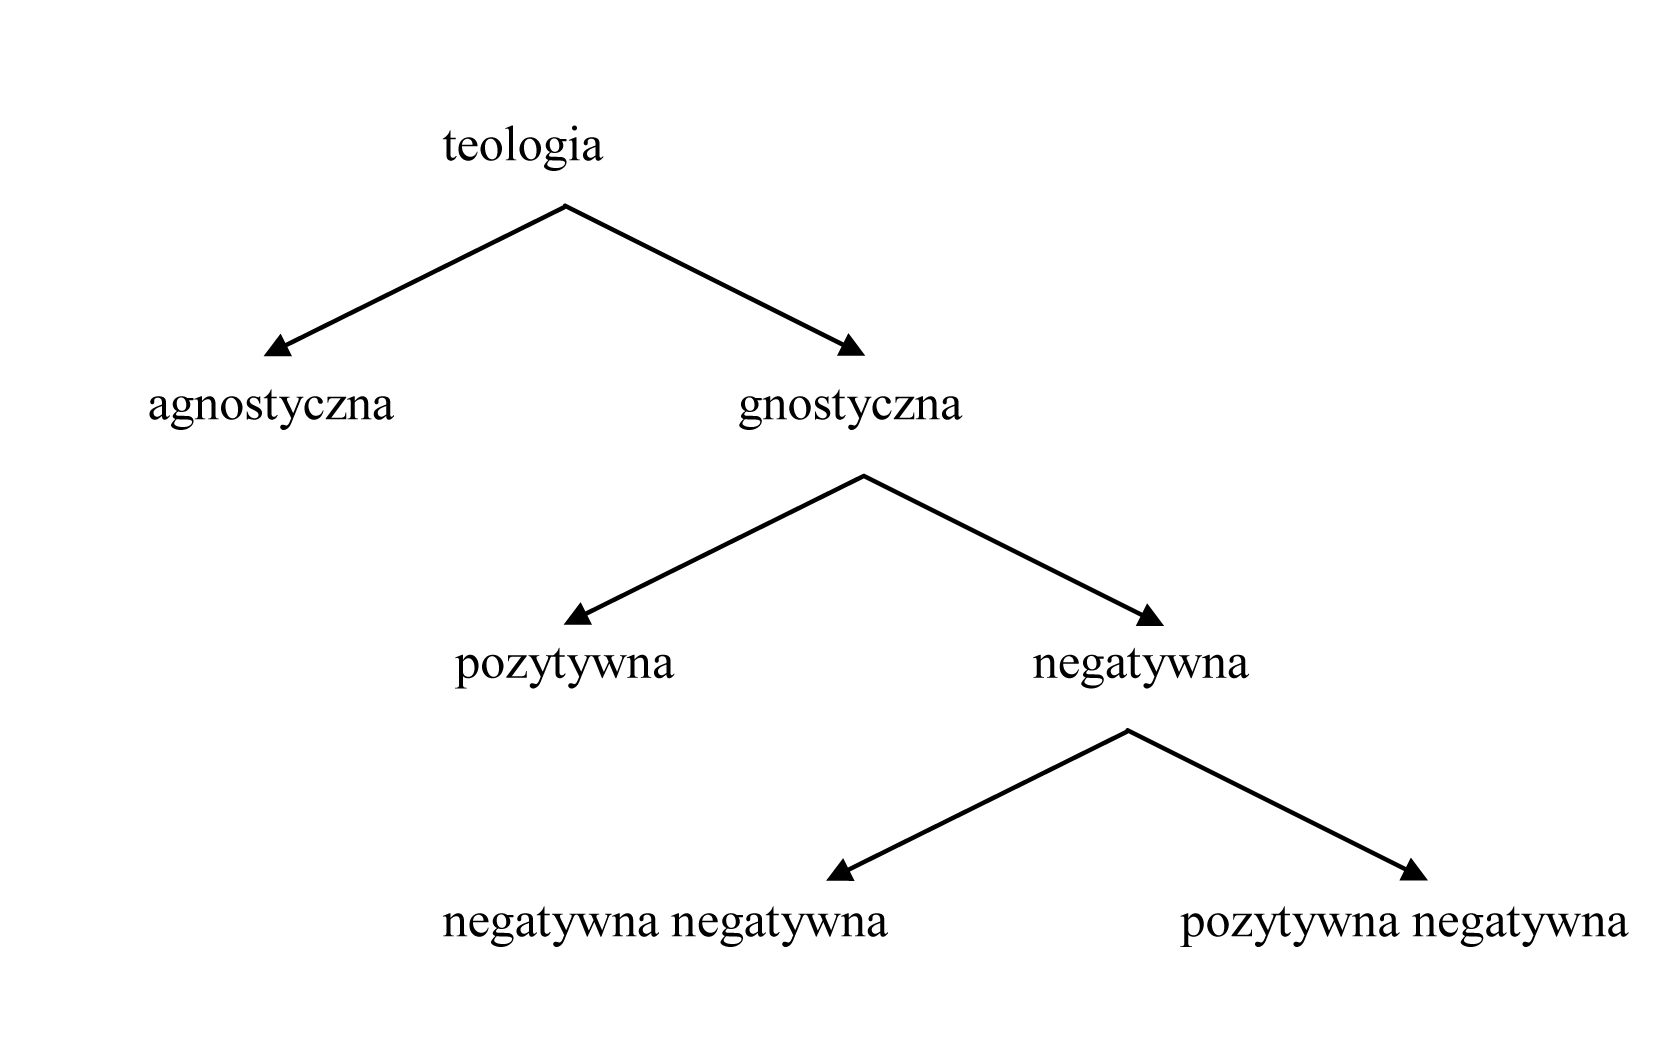
\includegraphics[width=1\linewidth]{typologia.jpg}
\caption{Proponowana przez Rojka
typologia interpretacji teologii apofatycznej.}
}
\end{figure}

Problemem, któremu Rojek poświęca nieco uwagi, lecz mimo wszystko
postanawia go nie rozstrzygać, jest problem własności pozytywnych. Jest
to problem poważny, ponieważ w świetle przedstawionej powyżej typologii
różnica między teologią pozytywną i negatywną polega na orzekaniu o
najwyższej istocie pozytywnych własności lub ich negacji. Jak
zdefiniować zbiór takich własności? Rojek wymienia kryterium
syntaktyczne, które miałoby polegać na „obecności negacji w
predykacie”\footnote{Tamże, s. 221. }. Nie do końca wiadomo, jak
rozumieć takie kryterium. Przypuszczam, że formalnie można zapisać tę
propozycję w logice predykatów II-rzędu w następujący sposób:

\begin{equation}
    P(Q) {=}_{df} \forall x \neg \exists N (Q(x) \equiv \neg N(x)),
\end{equation}
gdzie $P(Q)$ oznacza „własność $Q$ jest pozytywna”. Jednakże Rojek
natychmiast dodaje, że kryterium syntaktyczne nie może być uważane za
wystarczające. Powołuje się tu na klasyczny przykład predykatu „jest
ślepy” -- nie zawiera on negacji, lecz odnosi się do braku i z tego
powodu wydaje się być pozytywny. Trafniejszym argumentem wydaje się być
powołanie na św. Tomasza, wedle którego własności tradycyjnie
przypisywane bytowi absolutnemu, takie jak prostota, doskonałość czy
jedność, są w istocie własnościami negatywnymi\footnote{św. Tomasz z
Akwinu Teologiczna: I, 3, Summa contra Gentiles 11. }.

Problem własności pozytywnych Rojek pozostawia nierozwiązany tłumacząc,
że skupia się na formie teologii negatywnej, nie na jej treści. Dodaje
jednak, że istnieje jeszcze jeden bardzo szczególny sposób ich
rozumienia. Można je traktować, jako najwyższy sposób istnienia danej
własności, czyli tzw. perfekcje. Najczęściej mówi się o takich
perfekcjach, jak wszechwiedza -- najwyższy sposób wiedzy, czy też
wszechmoc -- najwyższy stopień mocy. Są one istotnym elementem w
ontologicznych dowodach istnienia Boga, które w historii były
proponowane m.in. przez św. Anzelma, Kartezjusza, Leibniza, Gödla i
Perzanowskiego. W tych argumentach Boga można uznać za podmiot
wszelkich własności pozytywnych rozumianych jako perfekcje:

\begin{equation}
    G(x) \equiv \forall Q (P(Q) \to Q(x)).
\end{equation}


Definicję tę Rojek zaczerpnął od Perzanowskiego\footnote{J.
Perzanowski, Ontological Arguments II: Cartesian and Leibnizian, [w:]
red. H. Burkhardt, B. Smith, Handbook of Metaphysics and Ontology, t.
2, PhilosophiaVerlag, München 1991,ss.~625–633. } i stanowi ona
wzór kolejnych definicji Boga w proponowanych przez niego następnie
interpretacjach teologii negatywnej. Warto wiec poświęcić jej nieco
uwagi. Po pierwsze, jest ona zapisana w rachunku predykatów drugiego
rzędu, gdyż zawiera warunek, że własności przypisywane Bogu muszą być
pozytywne. Po drugie, Bóg formalizowany jest jako predykat („$x$ jest
Bogiem”, „$x$ jest bogopodobny”), nie jako stała logiczna\footnote{Por.
choćby M. Durrant, The „Meaning of ‘God’-I, Royal Institute of
Philosophy Supplement,vol. 31 (1992), ss. 71-84. }, lub deskrypcja
określona, co proponował Bocheński\footnote{J.M. Bocheński, dz. cyt.,
s. 381. }. Po trzecie, powyższa definicja powstała na użytek
formalizacji dowodów ontologicznych, które należą raczej do jakiejś
formy teologii pozytywnej. Zawarte w niej $P(Q)$ czytamy jako „$Q$ jest
własnością pozytywną” w pewnym szczególnym sensie opisanym powyżej -- „$Q$
jest perfekcją”. Rojek nie sugeruje jednak, że w teologii apofatycznej
Pseudo-Dionizego zaprzecza się jedynie tego typu własnościom
pozytywnym. Przeciwnie, pisze wprost, że zakres negowanych własności
jest szerszy\footnote{P. Rojek, dz. cyt., s. 222. }. Po raz
kolejny jednak odżegnuje się od określenia, o jakie konkretnie
własności chodzi. Jest to, moim zdaniem, jeden z najsłabszych punktów
jego propozycji. Wrócę do tego ponownie w dyskusji.


\subsection{Agnostyczna teologia negatywna}

Strategią pierwszej przedstawianej przez Rojka interpretacji teologii
negatywnej jest przyjęcie (T4) jako tezy podstawowej i odrzucenie lub
modyfikacja pozostałych tez, za cenę zachowania spójności teorii.
Według tej interpretacji, celem teologii negatywnej jest wskazanie
boskiej transcendencji -- głosi ona, że Bóg jest zasadniczo
niepojmowalny i niewyrażalny.

Takie rozumienie teologii negatywnej jest popularne wśród wielu
komentatorów -- także tych, którzy rozważają logiczno-językową strukturę
tej teorii. Wśród nich Rojek wymienia Michaela Gellmana, Johna J.
Jonesa oraz Paula Rorema.

W rozważaniach Gellmana teologia negatywna jest teorią, w której
jakikolwiek predykat P języka „skończonych bytów” nie może być
przedziwie orzekany o Bogu. Jej główną tezą jest, że Bóg nie należy do
zakresu żadnego z predykatów naszego języka. Jeśli mówimy na przykład,
że Bóg nie jest mądry, mamy na myśli raczej negacją
\textit{wykluczającą}, niż negację \textit{wyboru}. Naszym zamiarem
jest wyłącznie stwierdzenie, że to nieprawda, że predykat P przysługuje
Bogu, niekoniecznie sugerując, że można o nim orzec dopełnienie tego
predykatu, czyli nie-P\footnote{J.I. Gellman, The Meta-Philosophy of
Religious Language. „No\^us”, nr 11 (1971), s. 158. }. Według
Gellmana, zdanie „Bóg jest potężny” teolog negatywny zrozumie jako
negację dopełnienia predykatu „jest potężny”. W innym kontekście
oznaczałoby to przypisanie obiektowi, o którym mowa, tej właśnie
własności. Jednakże w przypadku Boga negowanie dopełnienia predykatu P
nie oznacza przypisywania mu P. Mówiąc ogólnie, zdania języka
religijnego negują dopełnienia wszystkich wymienianych przez nie
własności Boga, który jest poza zakresem wszystkich naszych predykatów.
One, z kolei -- będąc predykatami języka skończonych bytów -- z
konieczności muszą oznaczać niedoskonałe własności\footnote{Zob.
Tamże. }.

Według Jonesa, teologia negatywna Pseudo-Dionizego Areopagity jest w
dużej mierze teologią krytyczną. Polemizuje ona z błędnym sposobem
mówienia o Bogu -- takim, który traktuje Go jak byty, czyli rzeczy lub
pojęcia\footnote{J.J. Jones, dz. cyt., s. 357. }. Fakt, że Bóg
przekracza wszelki byt, nadaje również strukturę językowi dyskursu
teologicznego. Nie idzie tylko o to, że przypisywanie Bogu
jakichkolwiek przymiotów przysługujących bytom jest z gruntu błędne.
Zwykle, gdy mówimy o rzeczach, twierdzenia i przeczenia sprzeciwiają
się sobie. W wykładni Dionizego nie dzieje się tak w przypadku Boga.
Bóg nie jest jednym z bytów, zatem język służący do opisu bytów nie
jest dla Niego właściwy. W wypracowanym przez niego języku teologicznym
twierdzenia i zaprzeczenia należą do odmiennych grup, tworząc odmienne
sposoby mówienia o Bogu. Ponieważ funkcjonują one w odmienny sposób,
nie należy ich ze sobą mieszać. Te pierwsze przedstawiają Boga jako
przyczynę wszystkiego, te drugie wyrażają jego transcendencję. Oba
sposoby mówienia można stosować naraz zarówno do opisu Boga, jak i
opisu przedmiotów, jednakże w ten sposób nie zdołamy wyrazić
unikalności Boga -- tego, że jest czymś odrębnym od wszystkich
bytów\footnote{Zob. Tamże, s. 360. }. Możemy tego dokonać
wyłącznie przez negację, która według Jonesa jest kluczowym punktem
myśli Dionizego. Istotnym jest, że Jones wyraźnie odróżnia negację od
zaprzeczenia.


\begin{quote}
        W przeciwieństwie do zaprzeczenia, negacja odnosi się do (nie)możliwości
poznania i powiedzenia czegokolwiek o Bogu. Jest to, jeśli można tak
powiedzieć, reguła drugiego rzędu posługiwania się nazwami pierwszego
rzędu.\footnote{Tamże, s. 381. Większą część tego cytatu podaję za
Rojkiem, dz. cyt., s. 222. }
\end{quote}






Najbardziej agnostyczną interpretację dionizyjskiej teologii negatywnej
zaproponował Paul Rorem. Podkreśla on podobieństwo teologii
Pseudo-Dionizego z późną filozofią neoplatońską. W obu tych doktrynach
byty uporządkowane są względem pewnej hierarchii i w celu dotarcia do
bytu absolutnego należy „wspiąć się” po tej „drabinie” bytów. By
spotkać Boga należy wpierw zanegować nasze wrażenia i wyobrażenia i
przekroczyć je, by dojść do ich pojęciowych znaczeń. Następnie
zanegowane zostać powinny także owe znaczenia oraz wszelkie inne
pojęcia umysłu, ponieważ przekroczenie naszej wiedzy prowadzi do
niepoznawalnego, do cichego zjednoczenia z Bogiem. Innymi słowy, Rorem
zwraca uwagę, że u Areopagity drogą do Boga jest zaprzeczenie
wszystkich bytów. Dionizy jednak wielokrotnie stwierdza, że Bóg jest
także ponad wszelkim zaprzeczeniem. Ostatecznie więc, należy zanegować
także wszelkie negacje, nie pozostawając już żadnym pojęciem
Boga\footnote{Por. P. Rorem, Pseudo-Dionysius. A Commentary on the
Texts and an Introduction to Their Influence, Oxford University Press,
Oxford -- New York 1993, ss. 210-211. }. Jak zauważa Rorem, Dionizy
„zaprzecza i wykracza poza wszystkie nasze pojęcia lub «pojęciowe»
atrybuty Boga i kończy na odrzuceniu wszelkiego mówienia i myślenia,
nawet negatywnego”\footnote{Tenże, przypis do Pseudo-Dionizy
Areopagita, The Complete Work, tłum. C. Luibheid,. Paulist Press, New
York 1987, s. 99. Cytuję za P. Rojek, dz. cyt. }.

Przedstawione powyżej prace pozwalają sądzić, że wynikiem agnostycznej
interpretacji teologii negatywnej nie jest zatem teza, że Bóg posiada
własności negatywne, lecz twierdzenie, że jest On niepoznawalny i
niewyrażalny. Zgodnie ze wskazaną w ten sposób dwuznacznością tezy (T4)
Rojek wyróżnia dwie wersje tej teorii. Wedle pierwszej z nich, Bóg jest
niewyrażalny, nie sposób Go wysłowić. Konsekwentnym rozwinięciem tej
teorii jest stwierdzenie, że dyskurs religijny jest pozbawiony
jakiegokolwiek znaczenia. Wedle drugiej wersji, Bóg jest tylko
niepoznawalny, nie można posiąść o nim wiedzy. I choć dyskurs religijny
posiada w tej teorii jakieś znaczenie, może on opisać wyłącznie to,
czego o Bogu nie wiemy. Rojek omawia obie wersje tej interpretacji.



\subsubsection{Teoria Niewysławialnego}

Według wielu komentatorów ta wersja agnostycznej teologii negatywnej
jest wewnętrznie sprzeczna. Z reguły argumentacja polega na wskazaniu,
że teoria ta twierdząc, że nie da się niczego powiedzieć o Bogu, sama
coś o Nim mówi, a zatem jest sprzeczna. W takim wypadku należałoby ją
odrzucić. Jednym krytyków teorii Niewysławialnego\footnote{Rojek używa terminu „Niewyrażalny”. W
niniejszej pracy pozostaje przy terminologii polskiego przekładu pracy
Bocheńskiego, Logika i teologia, dz. cyt. } jest Michael Durrant.
Pisze on, że

\begin{quote}
    w tej teorii, mówiąc, że natura Boga jest zasadniczo niewyrażalna,
opisujemy właśnie naturę Boga -- jest mianowicie zasadniczo
niewyrażalna. Innymi słowy, ci, którzy bronią tego stanowiska, nie mogą
tego robić nie przecząc sobie.\footnote{M. Durrant, The Meaning of
‘God’ (I). [w:] Religion and Philosophy, red.  M. Warner, Cambridge
University Press, Cambridge 1992, s. 74. Cytuję za P. Rojek, dz. cyt.,
s. 222-223. }
\end{quote}


Podobnie argumentuje John Hick, który uważa, że nie ma sensu


\begin{quote}
mówić o X, że żadne nasze pojęcie się do niego nie stosuje. Jest bowiem
w oczywisty sposób niemożliwe odnosić się do czegoś, co nie posiada
nawet własności 'bycia możliwym przedmiotem
odniesienia.\footnote{J. Hick, An Interpretation of Religion. Human
Responses to the Transcendent, Yale University Press, New Haven –
Londyn 1989, s. 239. Cytuję za P. Sikora, Logos Niepojęty, Wydawnictwo
Universitas, Kraków 2010, s. 118. }
\end{quote}


Dodaje on także, że określenie

\begin{quote}
,,taki, że nasze pojęcia się do niego nie stosują'' nie może,
jeśli chcemy uniknąć paradoksu, odnosić się do własności, którą
opisuje.\footnote{Tamże. }
\end{quote}

Przeciwko takiemu przedstawianiu teorii Niewysławialnego występuje Józef
Maria Bocheński. Twierdzi on, że da się ją uratować od sprzeczności,
lecz nawet mimo tego, nie odpowiada ona potrzebom dyskursu
religijnego\footnote{Zob. J.M. Bocheński, dz. cyt., ss. 353-356.
}. Bocheński uważa, że jeśli przestrzega się pewnych obowiązujących w
logice konwencji, zarzut sprzeczności stawiany teorii Niewysławialnego
przestanie obowiązywać. Należałoby wpierw dowieść, że danym układzie
odniesienia teoria ta prowadzi do sprzeczności, tymczasem nikt takiego
dowodu nie przedstawił. Według Bocheńskiego sytuacja przedstawia się
zupełnie przeciwnie -- nietrudno wykazać, że teoria Niewysławialnego
jest spójna. Poniżej przedstawię jego argumentację.

Załóżmy, że dwuargumentowy predykat  $Nw(x,l)$ oznacza „$x$ jest
niewyrażalne w języku $l$”.

Zapiszmy teraz formułę zawierającą ten predykat

\begin{equation}
    \exists x \exists l Nw(x, l)
\end{equation}


Wydaje się, że nie tylko można ją wypowiedzieć nie popadając w
sprzeczność, lecz także jest ona prawdziwa, nietrudno znaleźć taki
obiekt $x$ i taki język $l$, które spełniałyby zapisany wyżej warunek.
(Bocheński podaje przykład krowy i języka szachów: nie da się opisać
krowy w języku szachów).

Możemy powyższy przykład uogólnić i sformułować metajęzykową definicję
Boga o następującej postaci:

\begin{equation}\tag{G2}
    G(x) \equiv \forall l Nw(x, l)\footnote{Definicję podaję za
Rojkiem, różni się ona od zapisu Bocheńskiego tym, że u tego ostatniego
„Bóg” zapisany został jako stała logiczna: $\forall l Nw(a, l)$.}
\end{equation}



Na pierwszy rzut oka, wydaje się, ze ta formuła jest bardziej
problematyczna -- twierdzenie, że $x$ jest niewysłowione w żadnym języku
zdaje się prowadzić do sprzeczności. Można jednak uniknąć tego
problemu, stosując zwykłe konwencje wykorzystywane do pozbywania się
antynomii semantycznych. Należy założyć, że żadne zdanie traktujące o
pewnej klasie języków, nie jest formułowane w żadnym z tych języków.
Aby było pozbawione sprzeczności musi zostać sformułowane w innym
języku, czyli odpowiednim metajęzyku. Możemy więc założyć, że klasa
języków wspominana w (G2) jest klasą języków przedmiotowych. W takim
wypadku (G2) jest zdaniem metajęzyka pierwszego stopnia. Po takim
zabiegu, sformułowana definicja jest znacząca i pozbawiona
sprzeczności. Nie ma bowiem niespójności w twierdzeniu, że coś nie daje
się wysłowić w jakimś języku, lub nawet w klasie języków, o ile
twierdzenie to jest w języku nienależącym do tej klasy. Według
Bocheńskiego, przy takim założeniu, standardowym z punktu widzenia
logiki ogólnej, teoria Niewysławialnego pozostaje znacząca i spójna a
zarzut sprzeczności zostaje oddalony.

Bocheński odrzuca jednak teorię Niewysławialnego z co najmniej dwóch
powodów. Po pierwsze, na mocy (G2) nie można przypisać Bogu
jakiekolwiek własności językowo przedmiotowej. Jedyną własnością, jaką
możemy mu przypisać, jest metajęzykowa własność bycia niewysłowionym w
żadnym z języków przedmiotowych. W takim wypadku wierny, nie mógłby
akceptować żadnego zdania dyskursu religijnego, które przypisałoby Bogu
jakąkolwiek własność-przedmiotowo-językową. Wydaje się to niespójne z
faktycznym dyskursem religijnym. Po drugie, niemożliwe byłoby oddawanie
czci obiektowi, o którym wiemy tylko i wyłącznie, że nie można o nim
nic powiedzieć. Jeśli wierny miałby czcić obiekt pozbawiony własności
przedmiotowo-językowych, równie dobrze tym obiektem mógłby nie być Bóg
a szatan\footnote{Por. J.M. Bocheński, dz. cyt., ss. 354-356. }.

Rojek dodaje do tego podobny argument, jednakże umieszczony w kontekście
teologii negatywnej. Mianowicie, jeśli teoria Niewysławialnego ma być
właściwą interpretacją teologii negatywnej, można poddać w wątpliwość
zasadność jednoczesnego utrzymywania tez (T1)-(T3). Jeśli Bóg jest
niewyrażalny, cały język religijny jest pozbawiony znaczenia, nie
możemy więc ani sensownie potwierdzić, ani zaprzeczyć żadnym z Jego
własności. Dla Rojka jest to wskazówka, by (T4) nie interpretować
semantycznie, lecz epistemologicznie lub nawet ontologicznie\footnote{
Zob. P. Rojek, dz. cyt., s. 223. }. W ten sposób przechodzi się od
teorii Niewysławialnego do teorii Niepoznawalnego.


\subsubsection{Teoria Niepoznawalnego}

Teoria Niepoznawalnego jest lepszym modelem teologii apofatycznej,
ponieważ nie tylko przyjmuje (T4) za twierdzenie podstawowe, lecz także
umożliwia pewną interpretację tez (T2) oraz (T3).By to pokazać, Rojek
wprowadza pojęcie nieokreśloności oraz definiuje nowe, odmienne od
klasycznego pojęcie negacji. W tym celu wykorzystuje on logiczną teorię
nieokreśloności, którą na potrzeby modelowania filozofii nauki rozwinął
rosyjski logik, Aleksander Zinowjew\footnote{A. Zinowjew, Foundations
of the Logical Theory of Scientific Knowledge (Complex Logic), D.
Reidel Publishing Company, Dordrecht 1967. Zob. Także A. Zinowjew,
Logika nauki, tłum. Z. Simbierowicz, PWN, Warszawa 1976. }.

Zinowjew rozważa pewne nieklasyczne przypadki, do których nie można
zastosować prawa wyłączonego środka. Polegają one na przyjęciu
możliwości istnienia obiektów, co do których nie da się ustalić, czy
posiadają one jakąś własność $Q$, czy też posiadają własność
$\neg Q$. Takimi obiektami mogą być na przykład rozważana
w mechanice kwantowej cząstka elementarna, której parametry -- zgodnie z
zasadą nieoznaczoności -- nie mogą zostać ustalone, twierdzenie, które
na gruncie danego rachunku logicznego nie może zostać ani dowiedzione,
ani obalone, albo po prostu obiekt zmieniający się w czasie. Na
potrzeby tych przypadków wprowadźmy nowy funktor nieokreśloności i
oznaczmy go $?$\footnote{Dla utrzymania spójności zapisu, formuły teorii
nieokreśloności Zinowjewa przedstawiam w notacji zaproponowanej przez
Rojka, dz. cyt., s. 223.  }. Niech zapis $?Q(x)$ oznacza „nie można
ustalić, czy $Q(x)$, czy $\neg Q(x)$”, to znaczy „$x$ ma w sposób
nieokreślony $Q$”. Ponieważ w teorii Niepoznawalnego Bóg uznawany jest za
obiekt, którego nie da się poznać, za pomocą powyższego funktora możemy
podać nową definicję Boga, jako obiektu, który wszystkie swoje
własności posiada w sposób nieokreślony.

\begin{equation}\tag{G3}
   G(x) \equiv \forall Q (P(Q) \to ?Q(x)).
\end{equation}



Formule tej należy poświęcić nieco uwagi. Po pierwsze, w odróżnieniu od
(G2) powyższa definicja nie jest wyrażona w metajęzyku, lecz w języku
przedmiotowym. Po drugie, co istotniejsze, by uniknąć kłopotów z
formalizowaniem Boga przy użyciu predykatu $G(x)$, należy ją ograniczyć.
Do tej definicji trzeba dołożyć dodatkowe założenie, o postaci:

\begin{equation}
    \neg P(G)
\end{equation}


Innymi słowy, należy założyć, że predykat „jest Bogiem” (lub „jest
bogopodobny”) nie należy do zbioru predykatów pozytywnych. W
przedziwnym bowiem razie, wpadlibyśmy w błędne koło i o niczym nie
można byłoby określić, że jest Bogiem.

Jak zauważa Rojek, wykorzystując ten formalizm do modelowania teorii
Niepoznawalnego, można -- w pewnym szczególnym sensie -- zaprzeczyć, że
Bóg posiada wszystkie własności pozytywne. Oczywiście, nie idzie tutaj
o stwierdzenie, że o Bogu można na orzec jakiekolwiek
$\neg Q$, przy założeniu, że $Q$ jest własnością pozytywną.
Taki przypadek jest niezgodny definicją (G3). Idzie o to, że po
wprowadzeniu funktora nieokreśloności $?$, zdanie „nieprawda, że $x$ jest
$Q$”\footnote{Rojek mówi o wyrażeniu „$x$ jest nie-$Q$”, moim zdaniem
błędnie. Por. tamże. } staje się dwuznaczne. Może ono przyjąć jedno
z dwóch znaczeń: albo „$x$ jest nie-$Q$”, albo „nie można stwierdzić, czy $x$
jest $Q$”. W nomenklaturze Rojka, w pierwszym przypadku z zdaniu pojawia
się negacja w znaczeniu \textit{de re}, o drugim znaczeniu natomiast
można mówić, że zawiera ono negację \textit{de dicto}. Nieco inne
nazewnictwo wprowadził Zinowjew, który pierwszy rodzaj negacji nazwał
negacją wewnętrzną -- dotyczy ona bowiem wyłącznie predykatu, drugi
negacją zewnętrzną -- odnosi się ona bowiem do całego negowanego w ten
specyficzny sposób zdania.

Przyjmijmy teraz dwa różne symbole, w celu odróżnienia odmiennych pojęć
negacji. Niech $\neg$ oznacza negację \textit{de re},
natomiast symbol $\sim$ negację \textit{de dicto}. Przy
takiej notacji, formułę $\neg Q(x)$ czytamy jako „$x$ jest
nie-$Q$”, lub  inaczej: „$x$ ma własność nie-$Q$”\footnote{U Rojka: „$x$ ma
własność $\neg Q$”. }, natomiast formuła
$\sim\! Q(x)$\footnote{Rojek formułę, negowaną za pomocą
funktora $\sim$ opatruje w dodatkowe nawiasy po to, by
podkreślić odmienny, „zewnętrzny” charakter tego rodzaju negacji.
Uznaję ten zabieg za niekonieczny. Notacja Rojka jest odmienna od
stosowanej oryginalnie przez Zinowjewa. } oznacza „nie można
stwierdzić, czy $x$ jest $Q$”, lub  innymi słowy „nie jest twierdzi się, że
$x$ ma własność $Q$”. Poniższe aksjomaty definiują relacje, jakie zachodzą
pomiędzy funktorem nieokreśloności a funktorami negacji \textit{de re}
oraz negacji \textit{de dicto}:

\begin{equation}\tag{Z1}
\sim\! Q(x) \equiv ?Q(x) \lor \neg Q(x),
\end{equation}
\begin{equation}\tag{Z2}
\sim\!\neg Q(x) \equiv Q(x)\ \lor\ ?Q(x),
\end{equation}
\begin{equation}\tag{Z3}
\sim ?Q(x) \equiv Q(x) \lor \neg Q(x).
\end{equation}
Na ich podstawie można dowieść następujących tez:

\begin{equation}
   \vdash \quad ?Q(x)\ \equiv\ \sim\! Q(x)\ \land\ \sim\!\neg Q(x).
\end{equation}
 



Gdybyśmy chcieli dokonać kolapsu z powrotem do logiki klasycznej,
musielibyśmy przyjąć założenie, że negacje \textit{de re} i \textit{de
dicto} są wzajemnie definiowalne, to znaczy, że
$\neg Q(x) \equiv \sim\!Q(x)$. Jednakże, jeśli
chcemy opisać wspomniane wyżej przypadki nieklasyczne, w których
posiadanie lub nie posiadanie danej własności przez konkretny obiekt
nie może zostać określone, musimy zgodzić się na posiadanie dwóch
różnych, nierównoważnych pojęć negacji w systemie. Z tego powodu
poniższa formuła nie jest tezą prezentowanego rachunku:


\begin{equation}
    \nvdash \quad \sim\! Q(x) \to  \neg Q(x).
\end{equation}
Dzieje się tak, ponieważ $\sim\!Q(x)$ pociąga za sobą $\neg Q(x)$ lub
$?Q(x)$. Analogicznie, w prezentowanym tu rachunku nie zachodzi
następująca wersja prawa podwójnej negacji



\begin{equation}
   \nvdash \quad  \sim\! (\neg Q(\textit{x})) \to  Q(\textit{x}),
\end{equation}
ponieważ $\sim\!\neg Q(x)$ implikuje $Q(x)$ lub $?Q(x)$. Prawdziwe są
natomiast następujące formuły:



\begin{equation}
    \vdash \quad \neg Q(x) \to  \sim\! Q(x),
\end{equation}
\begin{equation}
    \vdash \quad Q(x) \to  \sim\! \neg Q(x).
\end{equation}






Należy zauważyć, że w przypadka z nieokreślonością nie można także mówić
o klasycznym prawie wyłączonego środka


\begin{equation}
     \nvdash \quad Q(x) \lor \neg Q(x),
\end{equation}
ponieważ istnieje dodatkowa, trzecia możliwość - $?Q(x)$. Do grona tez tego
rachunku należy zatem następująca formuła:

\begin{equation}
    \vdash \quad Q(x) \lor  \neg Q(x) \lor  ?Q(x)
\end{equation}


Co ciekawe, prawo wyłączonego środka obowiązuje dla negacji \textit{de
dicto}:

\begin{equation}
    \vdash \quad Q(x) \lor  \sim\! Q(x),
\end{equation}
\begin{equation}
    \vdash \quad \neg Q(x) \lor  \sim\! \neg Q(x),
\end{equation}
\begin{equation}
\vdash \quad ?Q(x) \lor  \sim\! ?Q(x).
\end{equation}

Jak zauważył Rojek, rachunek Zinowjewa stworzony pierwotnie na potrzeby
formalizacji teorii naukowych jest przydatny także do modelowania
omawianej w tym paragrafie interpretacji teologii apofatycznej. Dzięki
jego własnościom, można przedstawić w nim w sposób niesprzeczny aż trzy
tezy wypreparowane z pism Pseudo-Dionizego Areopagity. Formalną wersją
tezy (T4) jest definicja Boga podana przez (G3). Negację, o której mowa
w (T2) można traktować, jako negację \textit{de dicto}, ponieważ
zgodnie z teorią niepoznawalności Boga, nie możemy stwierdzić, czy
posiada On jakieś własności. W takim podejściu, (T2) stwierdza, że o
Bogu można orzec zewnętrzne negacje wszystkich własności pozytywnych. A
zatem, w języku tego rachunku należałoby to zapisać w następujący sposób:



\begin{equation}
    G(x) \to  (\forall Q (P(Q) \to  \sim\!Q(x)).
\end{equation}



Co więcej, powyższa formuła jest bezpośrednią konsekwencją definicji
(G3) i (1), które jest jednym z praw tego rachunku. Ponieważ negacja
\textit{de dicto}, jest różna od negacji \textit{de re}, nie możemy
jednocześnie twierdzić, że Bóg posiada (wewnętrzną) negację wszystkich
pozytywnych własności, czyli, że można o nim orzekać każde nie-$Q$, o ile
$Q$ jest pozytywne. Dzieje się tak, ponieważ z obu tych formuł wynika
także


\begin{equation}
    G(x) \to  (\forall Q (P(Q) \to
\sim\!\neg Q(x)),
\end{equation}


którą Rojek uważa za formalną postać tezy (T3). Formuła ta zawiera
podwójne przeczenie, jednakże pierwsza negacja ma charakter \textit{de
dicto}, natomiast druga jest negacją \textit{de re}. Brzmieniem tej
formuły jest „Nie można stwierdzić, czy Bóg posiada wszystkie negacje
pozytywnych własności”.

W takim wypadku, wszystkie stwierdzenia Dionizego o tym, że Bóg nie jest
ani $Q$, ani nie-$Q$, na przykład że nie jest On „ani wielkością, ani
małością, ani równością, ani nierównością, ani podobieństwem, ani
niepodobieństwem”, „nie jest też niczym z niebytu ani czymś z
bytu”\footnote{Pseudo-Dionizy Areopagita, Teologia mistyczna, dz.
cyt., rozdział V. } itp.,  można z łatwością interpretować w
świetle powyższej formalizacji. Podobnie sformułowania Areopagity o
tym, że Bóg jest „ponad wszelkim twierdzeniem i ponad wszelkim
zaprzeczeniem”\footnote{Tamże. } można ująć w ramach
prezentowanego rachunku, jako koniunkcję warunków zawartych już w
formułach (8) i (9).


\begin{equation}
    G(x) \to  (\forall Q (P(Q) \to  \sim\!(Q(x)) \land
\sim\!\neg Q(x)).
\end{equation}



Jak zauważa Rojek, istnieje wyjątek od konsekwentnego stosowania tej
interpretacji. Nie można w ten sposób formalizować  twierdzeń, że Bóg
nie jest ani poznawalny ani niepoznawalny, ani określony, ani
nieokreślony. Taka treść predykatu $Q$ naraziłaby bowiem tę interpretację
na sprzeczność. Jednakże wydaje się, że żadne z dzieł Dionizego nie
zawiera podobnych sformułowań\footnote{Także Jones zauważa, że teza o
niepoznawalności Boga ma wyjątkowy charakter w pismach Dionizego i
nigdy nie występuje w podobnych parach. Zob. J.J. Jones, dz. cyt., s.
358. }. Jedynie (T1) nie znajduje swojego miejsca w powyższej
interpretacji, bowiem -- skoro Bóg jest niepoznawalny -- nie można o nim
nic sensownie stwierdzić.

Powyższe analizy pozwalają sądzić, że wykorzystując odpowiednie
narzędzia formalne można obronić przed sprzecznościami obie formy
agnostycznej teologii negatywnej -- zarówno teorię Niewysławialnego, jak
i teorię Niepoznawalnego. Ta druga wydaje się o tyle lepszą
interpretacją teologii Pseudo-Dionizego, o ile na jej gruncie można
przyjąć aż trzy z wypreparowanych z tekstu Areopagity tez. Teoria
Niewysławialnego ustępuje w tym zestawieniu  i obejmuje tylko jedną
tezę dionizyjskiej doktryny. Obie jednak zawodzą w interpretacji (T1) i
jak zauważył Bocheński -- są zasadniczo niespójne z faktycznym dyskursem
i praktyką religijną. Zgodnie z ich duchem, wierny nie mógłby
akceptować żadnych zdań dyskursu religijnego, które przypisują Bogu
jakieś własności. Tymczasem, każdy dyskurs religijny zawiera
przynajmniej kilka takich zdań. Poza tym, gdyby o Bogu nie można było
orzekać żadnych własności, nie mógłby On być przedmiotem czci\footnote{
Zob. J.M. Bocheński, dz. cyt., ss. 355-356.}.




\subsection{Negatywna teologia negatywna}

Wad tych pozbawiona jest druga interpretacja teologii negatywnej, którą
Rojek nazywa negatywną teologią negatywną. Jej punktem wyjścia jest
teza (T2). Na gruncie tej interpretacji nie twierdzi się ani, że
dyskurs religijny pozbawiony jest znaczenia, ani że Bóg jest
niepoznawalny. Uważa się natomiast, że o przedmiocie religijnym można
orzekać wyłącznie negatywne własności. Nie jest więc tak, że nic nie
wiemy o Bogu -- wiemy, że nie posiada on pozytywnych własności. Należy
przyznać, że jest to dość popularna interpretacja teologii
apofatycznej. Na przykład, do właśnie w taki sposób rozumianej teologii
negatywnej odnosił się Józef Maria Bocheński w dziele \textit{Logika
religii}.

W analizie Rojka, negację obecną w (T2) na gruncie tej interpretacji
należy traktować jako zwykłą, klasyczną negację. Jeśli przyjmiemy
logikę klasyczną, zachowujemy zasadę niesprzeczności. W konsekwencji,
tezy (T1) oraz (T3) muszą zostać odrzucone, jako niespójne z tezą
przyjętą tu za podstawową.

Wedle tej wersji teologii negatywnej, wszystko, co możemy orzec o Bogu,
posiada ściśle negatywny charakter. Na tym polega boska transcendencja.
Choć Bóg zatraca tutaj swój sprzeczny charakter (obecny w jakimś
stopniu w agnostycznej teologii negatywnej), wciąż pozostaje w jakimś
sensie niepoznawalny. Jedyne, co o Nim wiemy to jaki nie jest. Można
więc pokusić się także na próbę uwzględnienia tezy (T4) w obrębie
niniejszych analiz.

Rojek twierdzi, że w tym modelu teologii negatywnej właściwą definicją
Boga jest formalizacja tezy (T2) w obrębie klasycznego rachunku
predykatów II-rzędu. Bóg -- analogicznie do poprzednich definicji –
opisany jest jako obiekt, o którym można orzekać negacje wszystkich
pozytywnych własności:


\begin{equation}\label{G4}\tag{G4}
    G(x) \equiv  \forall Q (P(Q) \to
\neg Q(x)).
\end{equation}





Podobnie, jak poprzednie definicje, także formuła (G4), wymaga
wprowadzenia szeregu ograniczeń po to, by w proponowany model nie
wkradła się żadna sprzeczność. Pierwsze ograniczenia dotyczą zbioru
pozytywnych własności. Jak wspominałem wcześniej, Rojek nie podaje
żadnej definicji, ani kryterium wyróżniania własności pozytywnych ze
zbioru wszystkich własności. Czyni jednak na ten temat kilka uwag,
które w większym bądź mniejszym stopniu nawiązują do rozważań
Bocheńskiego

Po pierwsze, według Rojka, zbiór pozytywnych własności nie może zawierać
własności negatywnych. Szczerze powiedziawszy, nie jest do końca jasne
także to, jak Rojek rozumie pojęcie własności negatywnej. W tym wypadku
jednak mamy dość tradycyjną, syntaktyczną definicję tego pojęcia.
Własność negatywna, zwana czasem także własnością dopełniającą, jest
jedną z własności złożonych i stanowi po prostu negację własności. W
języku naturalnym pojęcie negacji własności wrażamy prze użycie
przedrostka \textit{nie}- (w języku łacińskim
\textit{non}-)\footnote{Zob. J. Paśniczek, Predykacja, Copernicus
Center Press, Kraków 2014. }. Wydaje się, że Rojek pojęcie
własności negatywnej rozumie w podobny sposób, twierdzi bowiem, że nie
stosując tego ograniczenia, doprowadzimy do orzekania o Bogu także
własności pozytywnych (co z kolei sugeruje, że jest on także bliski
stosowaniu syntaktycznej definicji własności pozytywnej -- jako
niezawierającej spójnika negacji). Według Rojka, jeśli nie wprowadzimy
tego ograniczenia, nasz model umożliwi pozytywne twierdzenia o Bogu,
bowiem w przyjętej tu logice klasycznej $\neg \neg Q$
implikuje $Q$. Ponadto uważa on, że dopuszczenie do
zaprzeczania własności negatywnych wprowadzi do systemu sprzeczność,
bowiem umożliwi orzekanie o Bogu zarówno $\neg Q$, jak i
$\neg \neg Q$\footnote{Myślę, że
konsekwencji tej można by uniknąć wprowadzając porządną definicję
własności pozytywnych. Niestety, jak już zostało wspomniane, nie
została ona podana. }. Jednakże dla Rojka syntaktyczne kryterium
wyróżniania własności pozytywnych nie jest satysfakcjonujące.
Alternatywą dla niego byłoby kryterium epistemologiczne, zaproponowane
przez Bocheńskiego\footnote{J.M. Bocheński, dz. cyt., s. 416. }.
Wedle tego kryterium własności pozytywne definiuje się indukcyjnie,
jako własności postrzegane bezpośrednio lub zapisywane za pomocą
formuł, zawierających wyłącznie symbole własności pozytywnych i terminy
logiki pozytywnej. Rojek zgadza się z Bocheńskim, że także takie
kryterium nie jest wystarczająco ścisłe. Nie zamierza jednak
rozwiązywać tego problemu i podawać odpowiedniej definicji\footnote{
Por. P. Rojek, dz. cyt., s. 226. }.

Po drugie, po raz kolejny należy wykluczyć predykat „jest Bogiem” ze
zbioru predykatów oznaczających własności pozytywne. Uznanie własności
bycia Bogiem za własność pozytywną doprowadziłoby do sprzeczności:

\begin{equation}
    G(x) \equiv \neg G(x).
\end{equation}


Wedle Rojka, twierdzenie „Bóg nie jest boski” należy przeinterpretować w
taki sposób, by w orzeczniku tego zdania nie znalazł się predykat $G(x)$,
który użyty jest w (G4), lecz wiązka pozytywnych własności zwykle
przypisywanych Bogu. W mojej opinii problem ten mógłby zostać
rozwiązany poprzez formalizowanie Boga przy pomocy stałej logicznej,
zamiast predykatu „$x$ jest Bogiem”.

Jeśli przyjmiemy wszystkie te ograniczenia na proponowaną powyżej
definicję Boga, możemy doprowadzić ten model do ciekawych filozoficznie
konsekwencji. Zgodnie z omawianą wcześniej interpretacją Johna J.
Jonesa, głównym celem Dionizego było wykazanie, że Bóg jest ponad
wszelkim bytem, w szczególności nie należy on do kategorii przedmiotów.
Według popularnego rozumienia przedmiotu, można traktować go jako
podmiot własności. Taką definicją posługiwał się na przykład Stanisław
Leśniewki, według którego coś jest przedmiotem, o ile istnieje jakaś
własność, którą można o nim orzec\footnote{Rojek powołuje się tu na
dwa źródła: J. Słupecki, Stanisław Leśniewski’s Calculus of Names,
„Studia Logica”, nr 3 (1955), ss. 7--76 oraz J. Perzanowski, The Way
of Truth, [w:] red. R. Poli, P. Simons, Formal Ontology, Kluwer
Academic Publishers, Dordrecht 1996, ss. 61--130. }:

\begin{equation}
    Ob(x) \equiv  \exists Q  (Q(x)).
\end{equation}


Jeśli uzupełnimy tę definicję o warunek, że każdy przedmiot powinien
posiadać nie jakąkolwiek, ale pozytywną wartość, otrzymamy następującą
modyfikację\footnote{W świetle stawianych na definicję (G4) ograniczeń
konieczność wprowadzania w tę definicję dodatkowego zastrzeżenia wydaje
się wątpliwa. }:

\begin{equation}\label{D4}\tag{D4}
    Ob(x) \equiv  \exists Q P(Q) \land  Q(x).
\end{equation}


Zgodnie z tak zmodyfikowaną definicję, Bóg nie należy do zbioru
przedmiotów, ponieważ nie może on posiadać żadnych pozytywnych
własności.

\begin{equation}
    \forall x (G(x) \to  \neg Ob(x))\footnote{U Rojka zmienna x nie jest związana
    żadnym kwantyfikatorem}.
\end{equation}


Rojek konkluduje, ze gdy przyjmiemy powyższe rozważania za dobrą monetę,
Bóg istnieje w jakiś inny sposób, odmienny od tego, jak istnieją inne
byty. Według niego można tu mówić o istnieniu w sensie Quine’a (w
przeciwieństwie do istnienia w sensie przedmiotów Leśniewskiego).
Konkluzja ta zdaje się być w zgodzie z  rozważaniami tych zwolenników
teologii negatywnej, którzy podkreślają transcendencję Boga -- to, że
przekracza on wszystkie byty. W przedstawianym powyżej modelu nie można
Go bowiem traktować jako przedmiot w sensie uchwyconym w definicji
(D4).

Czy Bóg zdefiniowany za pomocą (G4) jest poznawalny? W jakimś sensie
możemy wyrazić jego naturę -- możemy mówić, jaki nie jest. Jednakże,
uczciwie rzecz ujmując, na gruncie tego modelu  nie możemy posiąść
żadnej pozytywnej wiedzy o Bogu. Z tego powodu w tej teorii znajdzie
się również miejsce na pewną interpretację tezy (T4). Rojek ujmuje ją w
następujący sposób:



\begin{quote}
    W normalnym wypadku rozumiemy natury rzeczy przez porównanie ich z tym,
czym one nie są. Jak mawiał Spinoza, „określenie jest negacją”. Bez
opozycji znaczeniowych i różnic nie moglibyśmy używać języka w sposób,
w jaki go faktycznie używamy. Bóg jako negacją wszelkich własności
znajduje się jednak poza całym systemem opozycji i różnic. Pełna
negacja prowadzi do całkowitego nieokreślenia.\footnote{P. Rojek, dz.
cyt., s. 226. }
\end{quote}




A zatem w pewnym sensie także na gruncie tej teorii możemy mówić o
niepoznawalności czy nawet niewyrażalności Boga.

Przedstawiony powyżej model teologii negatywnej -- o ile zgodzimy się na
wszystkie jego ograniczenia -- można uznać za logicznie spójny. Choć nie
uwzględnia on wszystkich tez wyabstrahowanych z dzieła Areopagity, w
atrakcyjny sposób rozwija on tezę o wyłącznie negatywnym charakterze
wiedzy o Bogu. Ponadto, nie wymaga on stosowania wyrafinowanych
narzędzi formalnych, pozostając przy logice klasycznej. Jego dodatkowym
atutem jest pewna interesująca filozoficznie własność -- Bóg rozumiany
jest tu jako istotnie odmienny od całej dziedziny bytów rozumianych
jako przedmioty. Jednakże w prezentowanym modelu nie ma miejsca na
interpretację tez (T1) oraz (T3). Ponadto, trudno go pogodzić z
dyskursem i praktyką religijną -- trudno jest bowiem oddawać cześć
czemuś, o czym wiemy tylko, czym nie jest\footnote{Jest to zarzut
stawiany przez Bocheńskiego, dz. cyt., s. 418. }.



\subsection{Pozytywna teologia negatywna}

Ostatnia interpretacja teologii negatywnej jest autorskim pomysłem
Rojka\footnote{Por. P. Rojek, dz. cyt., ss. 227-230. }. Również na
jej gruncie, podstawą tezą teologii negatywnej jest (T2). A zatem o
Bogu można orzec wyłącznie własności negatywne. Ponieważ model
stosowany do formalizacji tej interpretacji używa pewnego
specyficznego, nieklasycznego pojęcia negacji (innego niż wprowadzona
we wcześniejszych rozdziałach negacja \textit{de divto}), może on
również zinterpretować w odpowiedni sposób także tezy (T2) oraz (T3).
Model ten może również zawrzeć satysfakcjonującą interpretację tezy
(T4).

Punktem wyjścia interpretacji Rojka jest spostrzeżenie, że negacje w
pojawiające się tezxach teologii negatywnej Pseudo-Dionizego pełnią
specyficzną funkcję, odmienną od funkcji negacji klasycznej. Dionizy
zdawał sobie sprawę, że negacje, które stosuje nie należy rozumieć w
sensie braku (\textit{privatio}). Twierdził też, że w przypadku
wypowiedzi o Bogu „nie należy sądzić, że zaprzeczenia i twierdzenia
sprzeciwiają się sobie”\footnote{Pseudo-Dionizy Areopagita, dz. cyt.,
rozdział I, 2. }. Uznawał on więc możliwość jednoczesnego przyjęcia
zarazem twierdzenia o Bogu, jak i zaprzeczenie tego twierdzenia. Jak
zauważa Rojek, Dionizy wielokrotnie powtarza, że Bóg jest „powyżej”,
„poza” i „ponad” bytami lub że je „obejmuje”. Poniższy cytat jest
przykładem tego, jak Dionizy używał negacji:



\begin{quote}
    [Bóg] jest wszystkim jako przyczyna wszystkiego […]. I jest ponad
wszystkim, istniejąc ponadsubstancjalnie wcześniej niż wszystko, co
jest. Dlatego też wszystko na raz można o Nim twierdzić, choć On nie
jest żadną rzeczą.\footnote{Tamże, rozdział V, 8. }
\end{quote}





W obliczu takich sformułowań Rojek stwierdza, że dionizyjska negacja
oznacza jednoczesne zawieranie czegoś oraz byciu poza czy też ponad to
coś. W takim rozumieniu, negacja używana przez Areopagitę nie wyklucza
afirmacji. Rojek dodaje, że nawet jeśli tak rozumiane przeczenie nie
powinno się nazywać negacją, to zarzut stawiany Dionizemu nie powinien
polegać na oskarżaniu go o sprzeczność, tylko o niewłaściwe użycie
słów.

Rojek próbuje wykazać, że podobne rozumienie negacji można spotkać także
w języku potocznym. W tym celu posługuje się następującym przykładem:

\begin{quote}
    Załóżmy, że na stole leży 100 tysięcy zł w gotówce (nie jest to łatwe w
trakcie kryzysu). Załóżmy dalej, że ktoś pyta, czy na stole jest 10
groszy. Odpowiedź twierdząca byłaby oczywiście słuszna, lecz w pewien
sposób myląca. Wydaje się, że odpowiedź przecząca byłaby dopuszczalna,
a nawet bardziej wskazana. „Nie, ponieważ na stole leży o wiele, wiele
więcej niż 10 groszy”. Słowo „nie” nie oznacza w tej odpowiedzi
klasycznej negacji, lecz wyraża nieadekwatność supozycji pytania do
zachodzącego stanu rzeczy. Odpowiedź „tak” na to pytanie sugerowałaby,
że suma na stole jest w jakiś sposób porównywalna z 10 groszami. Taka
sama sytuacja zachodzi w wypadku takich pytań jak: „Czy Jan jest
zwierzęciem” („Nie! Jest człowiekiem!”), „Czy Romeo lubi Julię?” („Nie!
On ją kocha!”) itd.\footnote{P. Rojek, dz. cyt., s. 227. }
\end{quote}






Można mnożyć analogiczne przykłady. W podobnym duchu można stwierdzić,
że na obiedzie u teściowej na pytanie „Czy zupa była dobra?” dużo
lepiej (i bezpieczniej) jest odpowiedzieć „Nie, była pyszna!”.
Przykłady te wskazują, że w pewnych wypowiedziach  języka naturalnego
używamy zaprzeczeń, które polegają na klasycznej negacji logicznej. Jak
zauważa Rojek, przeczenie to ma również pozytywny, nie tylko negatywny
charakter i wyraża nie brak, ale nadmiar. Ponadto, uważa on, że takie
użycie przeczenie nie narusza reguł konwersacyjnych Grice’a, w
szczególności reguły ilości, która zabrania przekazywania większej
ilości informacji niż jest to konieczne. Informacja o tym, że dany
obiekt jest czymś większym, niż sądzi rozmówca, w pewnych kontekstach
wydaje się niezbędna. Nawet gdyby reguła ilości została naruszona,
zarzut ten jest dużo słabszy od zarzutu popadania w
sprzeczność\footnote{Zob. tamże. }.

W celu uzasadnienia stosowności używania tego rodzaju „pozytywnej”
negacji Rojek podaje też jego przykłady z dyskursu filozoficznego.
Podobne rozumienie negacji można spotkać u Stróżewskiego, który
rozróżnia dwa rodzaje negacji: przekreślający oraz różnicujący. Ta
pierwsza usuwa negowaną rzecz, ta druga jedynie podkreśla różnicę i jej
rezultatem nie jest brak, lecz w zasadzie jakieś pozytywne
stwierdzenie\footnote{Por. W. Stróżewski, Z problematyki negacji, [w:]
Tenże, Istnienie i sens, Wydawnictw Znak, Kraków 1994,
s.~373--395. }. Podobnego sensu negacji Rojek doszukuje się także
w heglowskim terminie \textit{Aufhebung}, które zwykle tłumaczy się
jako negację lub zniesienie. Powołuje się on na cytat z Hegla, który
wskazuje na dwuznaczny charakter tego słowa:

\begin{quote}
    Należy pamiętać o podwójnym sensie niemieckiego słowa aufheben
(odkładać, ściągać). Aufheben znaczy, po pierwsze, usuwać, anulować,
stąd mówi się, że prawo czy instytucja zostały anulowane. Po drugie,
aufheben znaczy także zachować, i w tym sensie mówimy, że coś zostało
zachowane. Tego podwójnego użycia języka, który nadaje temu samemu
słowu znaczenie pozytywne i negatywne, nie należy traktować jako czegoś
przypadkowego, ani tym bardziej krytykować język za wywoływanie
zamieszania. Powinniśmy raczej dostrzec w tym spekulatywnego ducha
naszego języka, przekraczającego podziały nagiego, rozsądkowego
albo-albo.\footnote{G.W.F. Hegel, Logic. Being Part One of the
Encyclopaedia of the Philosophical Sciences, tłum. W. Wallace. Oxford
University Press, Oxford 1975, §96. Cytuję za P. Rojek, dz. cyt.,
s.~228. }
\end{quote}






Rojek podkreśla, że u Hegla to, co zostało zniesione
(\textit{aufgehoben}) nie znika, lecz zostaje zachowane w doskonalszej
postaci.

Przedstawione powyżej wywody pozwalają sądzić, że zarówno w języku
potocznym, jak i filozoficznym można stosować negację w ten
specyficzny, „pozytywny” sposób. Takie rozumienie negacji nie może być
tożsame z negacją używaną w klasycznych rachunkach logicznych. Według
Rojka, właśnie w takim sensie Dionizy stosował negację w swoich
dziełach. Areopagita nie chciał twierdzić, że Bóg nie posiada żadnych
własności, lecz że posiada je w wyższy, pełniejszy sposób.

Na potrzeby analizy swojej interpretacji teologii negatywnej, Rojek
wprowadza zarys syntaktyki rachunku logicznego, który operowałby na tym
specyficznym rozumieniu negacji w sposób formalny. Stwierdzenie, że $x$
pozytywnie nie ma $Q$ oznacza w nim, że $x$ ma $Q$ w pewien szczególny,
wyższy sposób. Niech sformułowanie $!Q(x)$ oznacza „$x$ pozytywnie nie ma
$Q$”, lub innymi słowy „$x$ ma pozytywną negację $Q$”. Znaczenie negacji
pozytywnej Rojek próbuje (częściowo) ustalić za pomocą następujących
aksjomatów\footnote{Zob. P. Rojek, dz. cyt., s.~228. }:


\begin{equation}\label{A1}\tag{A1}
    !Q(x) \to  Q(x),
\end{equation}
\begin{equation}\label{A2}\tag{A2}
    \neg (Q(x) \to !Q(x)),
\end{equation}
\begin{equation}\label{A3}\tag{A3}
    !!Q(x) \to  !Q(x).
\end{equation}


Z tych aksjomatów natomiast wynikają następujące tezy:


\begin{equation}
    \vdash \quad \neg Q(x) \to  \neg !Q(x),
\end{equation}
\begin{equation}
    \vdash \quad \neg (!Q(x) \to  \neg Q(x
\end{equation}



Rojek zdaje sobie sprawę, że przedstawiony przez niego rachunek ma
charakter szkicowy, jednakże zaznacza, że powyższe aksjomaty i tezy
wystarczają do zaproponowanej przez niego analizy dionizyjskiej
doktryny. A zatem, w tej interpretacji Bóg posiada wszystkie negacje
pozytywnych własności, lecz negacje rozumiane są właśnie w ten
specyficzny, „pozytywny” sposób:




\begin{equation}\label{G5}\tag{G5}
 G(x) \equiv  \forall Q (P(Q) \to  !Q(x)).
\end{equation}



Powyższa formuła w niniejszym modelu stanowi formalizację tezy (T2). Z
niej oraz z aksjomatu (A1) wynika




\begin{equation}
G(x) \to  \forall Q (P(Q) \to  Q(x)).
\end{equation}




Oznacza to, że Bóg posiada wszystkie pozytywne własności nie tylko w
wyższy, pełniejszy sposób, lecz także w zwykły sposób. Innymi słowy,
Bóg jest nie jest mądry (w pozytywnym sensie) i jest mądry,
(pozytywnie) nie jest dobry i zarazem jest dobry, itd. Jest to pierwszy
z przedstawianych modeli teologii negatywnej, który zawiera zarówno
interpretację tezy (T2), jak i (T1).

Dzięki wprowadzanej w aksjomacie redukcji negacji pozytywnych, można w
prezentowanym systemie bezsprzecznie orzec o Bogu pozytywne negacje
pozytywnych negacji wszystkich pozytywnych własności. Na gruncie tego
modelu możemy zatem sformułować tezę (T3) w następujący sposób:




\begin{equation}
G(x) \to  \forall Q (P(Q) \to  !!Q(x)).
\end{equation}




W końcu, w interpretacji Rojka znajdzie się także miejsce dla tezy (T4).
Teza o niepoznawalności Boga zawiera się bowiem we wprowadzonym
„pozytywnym” pojęciu negacji. Gdy orzeka się o Bogu pozytywną negację
jakiejś pozytywnej własności, twierdzi się, że nie tylko posiada On tę
własność, lecz także, że posiada On ją w pewien wyższy, pełniejszy
sposób. Istota niepoznawalności Boga polega na tym, że nie i wiemy co
to znaczy posiadać jakąś własność w taki sposób, w jaki posiada ją Bóg.



\begin{quote}
    Choć wiemy, że Bóg jest mądry, nie wiemy, na czym polega bycie mądrym w
wypadku Boga. Wiemy tylko, że jego mądrość jest czymś więcej niż ludzka
mądrość. Nasza niewiedza nie dotyczy jednak tego, że Bóg jest mądry,
lecz ogranicza się tylko do sposobu, w jaki Bóg posiada mądrość. Wiemy,
że Bóg jest Q, wiemy, że jest !Q, ale nie wiemy, co to dokładnie
znaczy.\footnote{Tamże, s.~229. }
\end{quote}





Rojek zwraca uwagę, że przedstawiona prze niego interpretacja teologii
apofatycznej jest zbliżona do rozwiniętej prze św. Tomasza z Akwinu
teorii analogii. Jest o tyle interesująca uwaga, o ile niektórzy
komentatorzy próbują doszukać się apofatycznych wątków także w teologii
Akwinaty\footnote{Zob. P. Sikora, dz. cyt., ss.~79-87, a także B.
Davies, Aquinas on What God is Not, [w:] red. B. Davies,. Thomas
Aquinas. Contemporary Philosophical Perspectives, Oxford University
Press Oxford 2002, ss.~227–242; J. Wissink, Two Forms of Negative
Theology Explained Using Thomas Aquinas, [w:] red. I. N. Bulhof, L.
Kate, Flight of the Gods. Philosophical Perspectives on Negative
Theology, Fordham University Press, Fordham 2000, ss.~100--120; F.
O'Rourke, Pseudo-Dionysius and the Metaphysics of
Aquinas, EJ. Brill, Leiden -- New York 1992. }. Teoria analogii
głosi, że predykaty orzekane o Bogu nie są ani jednoznaczne, ani
wieloznaczne, lecz analogiczne. Predykaty jednoznaczne mają to samo
znaczenie, predykaty wieloznaczne, tak jak homonimy, mają całkowicie
różne znaczenia. Wciąż istnieją spory, co do właściwej interpretacji
znaczeń terminów analogicznych, jednakże z grubsza  rzecz biorąc, przy
ich pomocy nie tylko wyrażamy to, co one oznaczają, lecz także
wskazujemy ponad to, co przez nie rozumiemy. W ten sposób możemy
orzekać o Bogu pewne własności, jednocześnie nie wiedząc do końca, w
jaki sposób te własności Mu przysługują. Według Rojka, sens teologii
negatywnej Areopagity jest identyczny -- Dionizego i Tomasza różni tylko
sposób wypowiadania się. Gdy Tomasz mówi, że Bogu dana własność
przysługuje w pewien wyższy sposób, Dionizy orzeka o Bogu (pozytywną)
negację tej własności. Zasadniczo jednak wyrażają oni tę samą
myśl\footnote{Por. P. Rojek, dz. cyt., s.~229-230. }.



\clearpage
\section{Uwagi krytyczne}

Rojek przedstawia trzy interpretacje teologii negatywnej i próbuje podać
ich spójne formalizacje. Wszystkie trzy opierają się na tezach
wypreparowanych z \textit{Teologii mistycznej} Pseudo-Dionizego
Areopagity, różnią się jednak zasobem tez, które potrafią niesprzecznie
zinterpretować.

Pierwsza interpretacja, nazwana agnostyczną, podana jest w dwóch
wersjach: jednej kładącej nacisk na niewyrażalność Boga, drugiej
podkreślającej Jego niepoznawalność. Teoria Niewysławialnego, mimo iż
została obroniona przed ciążącym na niej zarzutem sprzeczności, okazuje
się niezdolna do uchwycenia tez Dionizego z wyjątkiem tezy (T4).
Formalizacja teorii Niepoznawalnego zasadniczo wykorzystuje logikę
nieokreśloności -- rachunek stworzony przez Aleksandra Zinowjewa na
potrzeby ścisłego badania pewnych filozoficznonaukowych koncepcji.
Manewrując dwoma różnymi rodzajami negacji -- \textit{de re} oraz
\textit{de dicto} -- obejmuje ona swoim zasięgiem wszystkie dionizyjskie
tezy teologii negatywnej, z wyjątkiem (T1).

Druga, „negatywna” interpretacja teologii negatywnej zdołała wcielić
tezy (T2) oraz (T4), zasadniczo odrzucając jednak (T1) oraz (T3). Mimo,
iż jej formalizacja wykorzystuje jedynie logikę klasyczną, posiada ona
pewną interesującą własność. Na jej gruncie można stwierdzić, że Bóg
nie należy do kategorii przedmiotów, co wyraża pożądaną przez wielu
teologów negatywnych transcendencję Boga. Wydaje się jednak, że zarówno
teorie agnostyczne, jak i negatywna teologia negatywna nie są zgodne z
dyskursem religijnym i praktyką religijną. Poza tym, nie obejmując
swoim zasięgiem wszystkich tez Dionizego, nie mogą służyć za dobre
interpretacje rozwijanej przez niego teologii.

Wad tych pozbawiona jest ostatnia zaproponowana przez Rojka
interpretacja, którą nazywa pozytywną teologią negatywną. Jej szkicowa
formalizacja stanowi spójny model dla wszystkich czterech tez teologii
Psudo-Dionizego. Ponadto, jej treść jest zbliżona do ogólnie
przyjmowanej teorii analogii św. Tomasza z Akwinu. Według Rojka, za jej
przyjęciem przemawia dodatkowy argument -- pasuje ona do modelu
chrześcijańskiego, którym niepoznawalność Boga i jego transcendencja
wynika nie ze spekulacji, lecz z Objawienia, w którym Bóg sam siebie
określa jako ukryty.

Modele podane przez Rojka wzbudzają jednak wiele zastrzeżeń. Po
pierwsze, zachowują one spójność teologii negatywnej, jednak za cenę
wielu restrykcji i ograniczeń. Zostały one przeze mnie wymienione przy
omawianiu definicji przedmiotu religijnego w każdej z proponowanych
interpretacji.

Po drugie, Rojek (świadomie!) nie podaje żadnego satysfakcjonującego
kryterium pozytywności własności. Według Rojka, różnica między teologią
pozytywną a teologią apofatyczną polegać ma na orzekaniu o Bogu
pozytywnych bądź negatywnych własności. W takim razie, jaka jest między
nimi różnica? Które własności są pozytywne a które negatywne? Jak
stwierdza Rojek, kryterium syntaktyczne jest niewystarczające. Podaje
tu klasyczny przykład ślepoty -- predykat „jest ślepy” nie zawiera
negacji, jednakże wciąż odnosi się do braku czegoś, no jest naturalne i
czego się spodziewamy. Z tego powodu wydaje się on być własnością
negatywną. Klasyczni filozofowie taki przykład własności negatywnej
nazywali negacją w sensie braku (\textit{privatio}). Rojek dodaje, że
większość własności, które zwyczajowo przypisuje się bytowi absolutnemu
na gruncie filozofii Boga, posiada charakter negatywny. Wykazał to św.
Tomasz\footnote{Zob. np. św. Tomasz z Akwinu Teologiczna: I, 3. }.
Można próbować, tak jak robił to Bocheński próbować podać
epistemologiczne kryterium pozytywności własności. Na przykład, możemy
podać indukcyjną definicję takiej własności:

\begin{enumerate}
\item Bezpośrednio postrzegana własność jest własnością pozytywną.
\item Własność zdefiniowana przez formułę zawierającą włącznie symbole
własności pozytywnych i terminu logiki pozytywnej jest własnością
pozytywną.
\end{enumerate}
Jednakże, zarówno Bocheński, jak i Rojek odrzucają i takie kryterium,
jako niewystarczająco ścisłe. W ostateczności, zbiór własności
pozytywnych można podać przez wyliczenie. Jednakże w takim wypadku
wszystkie proponowane przez Rojka teorie będą miały mocno ograniczony
zakres. W każdym razie, jeśli ktoś próbuje ograniczyć zasięg danej
teorii do klasy własności pozytywnych, takie własności muszą zostać
zdefiniowane. Uważam to za najsłabszy punkt jego rozważań.

Problem ten dodatkowo pogłębia fakt, że Dionizy w żadnym miejscu wprost
nie stwierdza, że własności orzekane lub zaprzeczane o Bogu mają
pozytywny bądź negatywny charakter. Jest to terminologia wprowadzona w
tezy doktryny Areopagity przez samego Rojka. W obliczu tego faktu tym
bardziej dziwi, że celowo odżegnuje się on od podania stosownej
definicji wprowadzonych przez niego pojęć.

Po trzecie, w żadnej z przedstawionych interpretacji predykat „jest
Bogiem” (lub „jest bogopodobny”) nie może być własnością pozytywną. W
modelu teorii Niepoznawalnego prowadzi to do zaskakującej konsekwencji
– mianowicie jeśli coś jest Bogiem, to nie można ustalić, czy to jest
Bogiem, czy nie jest Bogiem. W modelu negatywnej teologii negatywnej z
uznania własności bycia Bogiem za pozytywną wynika zwykła sprzeczność.
Natomiast w modelu pozytywnej teologii negatywnej pozytywna własność
bycia Bogiem oznaczałaby, że jeśli coś jest Bogiem, to pozytywnie nim
nie jest, czyli posiada tę własność w wyższy, pełniejszy sposób.
Wszystkie te niedogodności spowodowane są sposobem, w jaki Rojek
formalizuje przedmiot religijny -- czynie to nie za pomocą stałej
logicznej (wtedy słowo „Bóg” traktowane byłby jak nazwa), lecz za
pomocą predykatu (w takim wypadku „Bóg” jest własnością).

Po czwarte, system formalny zaproponowany dla sformalizowania pozytywnej
teologii negatywnej, ma bardzo szkicowy i wstępny charakter. Ciężko w
jego przypadku mówić o rachunku logicznym, nie zaproponowano dla niego
żadnej semantyki, tym bardziej nie udowodniono jego trafności i
pełności. Można powiedzieć, że praca potrzebna do formalizacji tej
teorii a zatem także wykazanie jej niesprzeczności, została wykonana
jedynie częściowo, w zarysie. I jeśli chcemy mówić o spójności
pozytywnej teologii negatywnej, należałoby ją dokończyć.

Po wtóre, można powiedzieć, że teologia negatywna interpretowana przy
użyciu pojęcia „pozytywnej” negacji traci swój negatywny charakter i
staje się formą pozytywnej, afirmatywnej teologii\footnote{Por. S.
Ruczaj, Analogia i apofatyczny pazur, „Pressje”, nr 30/31 (2012),
ss.~280-282.}.

Wszystkie te zarzuty nie oznaczają jednak, że logika formalna jest
bezużyteczna w badaniu teorii i interpretacji teologii negatywnej.
Przeciwnie, uważam, że rekonstrukcja różnych wersji teologii
apofatycznej w terminach formalnych systemów logicznych może być
obustronnie korzystna. Z jednej strony, jak pokazał Rojek, może ona
podać spójne modele interpretacji, które obejmują wszystkie tezy
teologii negatywnej i tym samym pomóc w wyborze najlepszej z nich. Z
drugiej strony, badanie teologii negatywnej przy użyciu narzędzi
formalnych może pomóc w dostarczeniu pewnych formalnych kryteriów
podziału dla odmiennych pojęć negacji i zbadaniu relacji zachodzących
między nimi, co może okazać się korzystne dla logiki i jej filozofii.

